\PassOptionsToPackage{unicode=true}{hyperref} % options for packages loaded elsewhere
\PassOptionsToPackage{hyphens}{url}
%
\documentclass[
]{article}
\usepackage{lmodern}
\usepackage{amssymb,amsmath}
\usepackage{ifxetex,ifluatex}
\ifnum 0\ifxetex 1\fi\ifluatex 1\fi=0 % if pdftex
  \usepackage[T1]{fontenc}
  \usepackage[utf8]{inputenc}
  \usepackage{textcomp} % provides euro and other symbols
\else % if luatex or xelatex
  \usepackage{unicode-math}
  \defaultfontfeatures{Scale=MatchLowercase}
  \defaultfontfeatures[\rmfamily]{Ligatures=TeX,Scale=1}
\fi
% use upquote if available, for straight quotes in verbatim environments
\IfFileExists{upquote.sty}{\usepackage{upquote}}{}
\IfFileExists{microtype.sty}{% use microtype if available
  \usepackage[]{microtype}
  \UseMicrotypeSet[protrusion]{basicmath} % disable protrusion for tt fonts
}{}
\makeatletter
\@ifundefined{KOMAClassName}{% if non-KOMA class
  \IfFileExists{parskip.sty}{%
    \usepackage{parskip}
  }{% else
    \setlength{\parindent}{0pt}
    \setlength{\parskip}{6pt plus 2pt minus 1pt}}
}{% if KOMA class
  \KOMAoptions{parskip=half}}
\makeatother
\usepackage{xcolor}
\IfFileExists{xurl.sty}{\usepackage{xurl}}{} % add URL line breaks if available
\IfFileExists{bookmark.sty}{\usepackage{bookmark}}{\usepackage{hyperref}}
\hypersetup{
  pdftitle={UIN Malang Internet Addiction Analysis},
  pdfauthor={Mely Santoso},
  pdfborder={0 0 0},
  breaklinks=true}
\urlstyle{same}  % don't use monospace font for urls
\usepackage[margin=1in]{geometry}
\usepackage{color}
\usepackage{fancyvrb}
\newcommand{\VerbBar}{|}
\newcommand{\VERB}{\Verb[commandchars=\\\{\}]}
\DefineVerbatimEnvironment{Highlighting}{Verbatim}{commandchars=\\\{\}}
% Add ',fontsize=\small' for more characters per line
\usepackage{framed}
\definecolor{shadecolor}{RGB}{248,248,248}
\newenvironment{Shaded}{\begin{snugshade}}{\end{snugshade}}
\newcommand{\AlertTok}[1]{\textcolor[rgb]{0.94,0.16,0.16}{#1}}
\newcommand{\AnnotationTok}[1]{\textcolor[rgb]{0.56,0.35,0.01}{\textbf{\textit{#1}}}}
\newcommand{\AttributeTok}[1]{\textcolor[rgb]{0.77,0.63,0.00}{#1}}
\newcommand{\BaseNTok}[1]{\textcolor[rgb]{0.00,0.00,0.81}{#1}}
\newcommand{\BuiltInTok}[1]{#1}
\newcommand{\CharTok}[1]{\textcolor[rgb]{0.31,0.60,0.02}{#1}}
\newcommand{\CommentTok}[1]{\textcolor[rgb]{0.56,0.35,0.01}{\textit{#1}}}
\newcommand{\CommentVarTok}[1]{\textcolor[rgb]{0.56,0.35,0.01}{\textbf{\textit{#1}}}}
\newcommand{\ConstantTok}[1]{\textcolor[rgb]{0.00,0.00,0.00}{#1}}
\newcommand{\ControlFlowTok}[1]{\textcolor[rgb]{0.13,0.29,0.53}{\textbf{#1}}}
\newcommand{\DataTypeTok}[1]{\textcolor[rgb]{0.13,0.29,0.53}{#1}}
\newcommand{\DecValTok}[1]{\textcolor[rgb]{0.00,0.00,0.81}{#1}}
\newcommand{\DocumentationTok}[1]{\textcolor[rgb]{0.56,0.35,0.01}{\textbf{\textit{#1}}}}
\newcommand{\ErrorTok}[1]{\textcolor[rgb]{0.64,0.00,0.00}{\textbf{#1}}}
\newcommand{\ExtensionTok}[1]{#1}
\newcommand{\FloatTok}[1]{\textcolor[rgb]{0.00,0.00,0.81}{#1}}
\newcommand{\FunctionTok}[1]{\textcolor[rgb]{0.00,0.00,0.00}{#1}}
\newcommand{\ImportTok}[1]{#1}
\newcommand{\InformationTok}[1]{\textcolor[rgb]{0.56,0.35,0.01}{\textbf{\textit{#1}}}}
\newcommand{\KeywordTok}[1]{\textcolor[rgb]{0.13,0.29,0.53}{\textbf{#1}}}
\newcommand{\NormalTok}[1]{#1}
\newcommand{\OperatorTok}[1]{\textcolor[rgb]{0.81,0.36,0.00}{\textbf{#1}}}
\newcommand{\OtherTok}[1]{\textcolor[rgb]{0.56,0.35,0.01}{#1}}
\newcommand{\PreprocessorTok}[1]{\textcolor[rgb]{0.56,0.35,0.01}{\textit{#1}}}
\newcommand{\RegionMarkerTok}[1]{#1}
\newcommand{\SpecialCharTok}[1]{\textcolor[rgb]{0.00,0.00,0.00}{#1}}
\newcommand{\SpecialStringTok}[1]{\textcolor[rgb]{0.31,0.60,0.02}{#1}}
\newcommand{\StringTok}[1]{\textcolor[rgb]{0.31,0.60,0.02}{#1}}
\newcommand{\VariableTok}[1]{\textcolor[rgb]{0.00,0.00,0.00}{#1}}
\newcommand{\VerbatimStringTok}[1]{\textcolor[rgb]{0.31,0.60,0.02}{#1}}
\newcommand{\WarningTok}[1]{\textcolor[rgb]{0.56,0.35,0.01}{\textbf{\textit{#1}}}}
\usepackage{graphicx,grffile}
\makeatletter
\def\maxwidth{\ifdim\Gin@nat@width>\linewidth\linewidth\else\Gin@nat@width\fi}
\def\maxheight{\ifdim\Gin@nat@height>\textheight\textheight\else\Gin@nat@height\fi}
\makeatother
% Scale images if necessary, so that they will not overflow the page
% margins by default, and it is still possible to overwrite the defaults
% using explicit options in \includegraphics[width, height, ...]{}
\setkeys{Gin}{width=\maxwidth,height=\maxheight,keepaspectratio}
\setlength{\emergencystretch}{3em}  % prevent overfull lines
\providecommand{\tightlist}{%
  \setlength{\itemsep}{0pt}\setlength{\parskip}{0pt}}
\setcounter{secnumdepth}{-2}
% Redefines (sub)paragraphs to behave more like sections
\ifx\paragraph\undefined\else
  \let\oldparagraph\paragraph
  \renewcommand{\paragraph}[1]{\oldparagraph{#1}\mbox{}}
\fi
\ifx\subparagraph\undefined\else
  \let\oldsubparagraph\subparagraph
  \renewcommand{\subparagraph}[1]{\oldsubparagraph{#1}\mbox{}}
\fi

% set default figure placement to htbp
\makeatletter
\def\fps@figure{htbp}
\makeatother


\title{UIN Malang Internet Addiction Analysis}
\author{Mely Santoso}
\date{10/29/2020}

\begin{document}
\maketitle

\hypertarget{pendahuluan}{%
\section{\texorpdfstring{\textbf{Pendahuluan}}{Pendahuluan}}\label{pendahuluan}}

Saya berlatarbelakang lulusan jurusan psikologi dari UIN Malang.
Kesibukan saya saat ini yang paling utama adalah salat 5 waktu dan
mengajar mengaji

Data yang dianalisis ini terdiri dari dua kategori utama yaitu 1) data
demografi dan; 2) data psikologis

Mari terhubung di twitter
\href{https://twitter.com/himelysantoso}{himelysantoso} atau instagram
\href{https://www.instagram.com/melysantoso/}{melysantoso}

Jika Anda tertarik dengan tulisan berbasis data atau penjelasan berbasis
sains, coba tengok tulisan-tulisan user story saya di
\href{https://kumparan.com/melysantoso}{Kumparan} akhir-akhir ini
meliput COVID-19. Atau tulisan lain saya yang membahas psikologi di
\href{https://medium.com/@bukakurung}{Medium}

\hypertarget{persiapan-data-merapikan-dan-membersihkan-data-yang-tidak-dibutuhkan}{%
\subsection{\texorpdfstring{\emph{Persiapan Data (Merapikan dan
Membersihkan Data yang Tidak
Dibutuhkan)}}{Persiapan Data (Merapikan dan Membersihkan Data yang Tidak Dibutuhkan)}}\label{persiapan-data-merapikan-dan-membersihkan-data-yang-tidak-dibutuhkan}}

Data yang digunakan dalam analisis ini adalah data pribadi dari skripsi
saya Data ini dikumpulkan dari mahasiswa baru tahun 2018 lalu

\textbf{\emph{Catatan}}

\begin{itemize}
\tightlist
\item
  Untuk kepentingan kerahasiaan responden kita buang data yang bersifat
  privat seperti nama dan email
\item
  Variabel ``Asal'' tidak seberapa baik datanya jadi kita buang
\item
  Untuk mempelajari membuat kategorisasi di R, kita buang variabel
  ``Addicted''
\end{itemize}

\begin{Shaded}
\begin{Highlighting}[]
\CommentTok{#Import library()}
\KeywordTok{library}\NormalTok{(ggplot2)}
\KeywordTok{library}\NormalTok{(reshape2)}
\KeywordTok{library}\NormalTok{(tidyverse)}
\KeywordTok{library}\NormalTok{(dplyr)}
\KeywordTok{library}\NormalTok{(gridExtra)}
\KeywordTok{library}\NormalTok{(ggalluvial)}
\KeywordTok{library}\NormalTok{(treemapify)}
\KeywordTok{library}\NormalTok{(ggcorrplot)}
\KeywordTok{library}\NormalTok{(visreg)}
\KeywordTok{library}\NormalTok{(vcd)}
\KeywordTok{library}\NormalTok{(correlation)}

\CommentTok{# 1) IMPORT & DATA CLEANING}

\CommentTok{# a) Masukkan data }
\NormalTok{internetdata <-}\StringTok{ }\KeywordTok{read.csv}\NormalTok{(}\StringTok{"datainternet.csv"}\NormalTok{)}
\CommentTok{#View(internetdata) #untuk melihat data }
\CommentTok{#glimpse(internetdata) #tidy up nama-nama variable}
\CommentTok{#table(internetdata$Usia) #akses spesifik variabel}

\CommentTok{# b) Buang observasi yang bersifat private dan tidak dibutuhkan }
\NormalTok{internetdata <-}\StringTok{ }\NormalTok{internetdata }\OperatorTok
\StringTok{  }\KeywordTok{select}\NormalTok{(}\OperatorTok{-}\KeywordTok{c}\NormalTok{(}\StringTok{"Nama"}\NormalTok{, }\StringTok{"Email"}\NormalTok{, }\StringTok{"Asal"}\NormalTok{, }\StringTok{"Addicted"}\NormalTok{)) }\OperatorTok
\StringTok{  }\KeywordTok{as.data.frame}\NormalTok{()}

\CommentTok{# c) Beberapa data dijadikan nominal }
\NormalTok{data_nominal <-}\StringTok{ }\NormalTok{(}\KeywordTok{c}\NormalTok{(}\StringTok{"Sex"}\NormalTok{, }\StringTok{"Fakultas"}\NormalTok{, }\StringTok{"Pendidikan"}\NormalTok{, }\StringTok{"Device"}\NormalTok{, }\StringTok{"WiFi"}\NormalTok{, }
                   \StringTok{"Koneksi"}\NormalTok{, }\StringTok{"Alasan"}\NormalTok{, }\StringTok{"MedSos"}\NormalTok{, }\StringTok{"Lembur"}\NormalTok{, }\StringTok{"Layanan"}\NormalTok{,}
                   \StringTok{"Situs"}\NormalTok{, }\StringTok{"Waktu"}\NormalTok{, }\StringTok{"Tempat"}\NormalTok{))}
\NormalTok{internetdata[data_nominal] <-}\StringTok{ }\KeywordTok{lapply}\NormalTok{(internetdata[data_nominal], }\ControlFlowTok{function}\NormalTok{(x)\{}\KeywordTok{factor}\NormalTok{(x)\})}

\CommentTok{# d) Obs Durasi dijadikan ordinal aja biar bisa dianalisis }
\NormalTok{internetdata}\OperatorTok{$}\NormalTok{Durasi <-}\StringTok{ }\KeywordTok{factor}\NormalTok{(internetdata}\OperatorTok{$}\NormalTok{Durasi,}
                              \DataTypeTok{ordered =}\NormalTok{ T,}
                              \DataTypeTok{levels =} \KeywordTok{c}\NormalTok{(}\StringTok{"1- 3 Jam"}\NormalTok{,}
                                         \StringTok{"4 - 7 Jam"}\NormalTok{,}
                                         \StringTok{"> 7 Jam"}\NormalTok{)) }


\CommentTok{# 2) OTHER DATA ISSUEs}
\CommentTok{# Karena ini adalah data pengukuran psikologi maka ada beberapa hal yang harus dilakukan }

\CommentTok{#) a) Buat kategori kelompok adiksi dan non adiksi }
\NormalTok{internetdata}\OperatorTok{$}\NormalTok{Kategori <-}\StringTok{ }\KeywordTok{ifelse}\NormalTok{(internetdata}\OperatorTok{$}\NormalTok{IA }\OperatorTok{<=}\StringTok{ }\KeywordTok{round}\NormalTok{(}\KeywordTok{mean}\NormalTok{(internetdata}\OperatorTok{$}\NormalTok{IA)), }\StringTok{"nonadiksi"}\NormalTok{, }\StringTok{"adiksi"}\NormalTok{)}


\CommentTok{# Cek datanya}
\KeywordTok{glimpse}\NormalTok{(internetdata)}
\end{Highlighting}
\end{Shaded}

\begin{verbatim}
## Rows: 446
## Columns: 20
## $ Sex        <fct> Laki-laki, Laki-laki, Laki-laki, Laki-laki, Perempuan, Laki-laki, Laki-laki, Perempuan, Peremp...
## $ Usia       <int> 19, 19, 18, 19, 19, 18, 18, 18, 18, 18, 18, 18, 20, 17, 19, 18, 18, 20, 18, 18, 19, 18, 18, 19...
## $ Fakultas   <fct> FITK, FITK, FITK, FITK, FITK, FITK, FITK, FITK, FITK, FITK, FITK, FITK, FITK, FITK, FITK, FITK...
## $ Pendidikan <fct> MA, MA, SMA, Pondok Pesantren, MA, SMA, MA, Pondok Pesantren, MA, MA, Pondok Pesantren, MA, Po...
## $ Durasi     <ord> > 7 Jam, 4 - 7 Jam, 4 - 7 Jam, > 7 Jam, 4 - 7 Jam, 4 - 7 Jam, 1- 3 Jam, > 7 Jam, > 7 Jam, 4 - ...
## $ Device     <fct> Smart Phone, Smart Phone, Smart Phone, Smart Phone, Smart Phone, Smart Phone, Smart Phone, Sma...
## $ WiFi       <fct> Ada dong!, Ada dong!, Ada dong!, Ada dong!, Ada dong!, Ada dong!, Ada dong!, Ada dong!, Ada do...
## $ Koneksi    <fct> Paket Data, Paket Data, WiFi, Paket Data, WiFi, Paket Data, Paket Data, Paket Data, WiFi, WiFi...
## $ Alasan     <fct> Bersosialisasi, Bersosialisasi, Mengisi waktu luang, Terkait dengan tugas kuliah, Terkait deng...
## $ MedSos     <fct> WhatsApp, WhatsApp, Instagram, WhatsApp, WhatsApp, Instagram, WhatsApp, WhatsApp, WhatsApp, Wh...
## $ Lembur     <fct> Iya, Iya, Iya, Tidak, Tidak, Tidak, Tidak, Iya, Iya, Iya, Iya, Iya, Iya, Tidak, Iya, Iya, Iya,...
## $ Layanan    <fct> "Browsing", "Chatting", "Media Sosial", "Nonton vidio", "Media Sosial", "Media Sosial", "Chatt...
## $ Situs      <fct> "Gramedia", "Facebook.com", "Seni ", "Wikipedia", "Berita terkini", "Instagram, Wikipedia, pem...
## $ Waktu      <fct> Menunggu sesuatu (contoh : menunggu dosen), Menjelang tidur, Kapanpun asal ada akses internet,...
## $ Tempat     <fct> Kamar, Kamar, Kamar, Kalau lagi boring, Kamar, Dimanapun asal ada akses internet, Kamar, Kamar...
## $ IA         <int> 21, 40, 86, 18, 13, 23, 36, 2, 54, 40, 47, 29, 54, 20, 34, 55, 45, 66, 50, 56, 20, 47, 38, 24,...
## $ Depresi    <int> 14, 18, 19, 2, 2, 0, 41, 1, 0, 0, 9, 4, 10, 36, 4, 8, 8, 9, 16, 14, 20, 6, 0, 4, 5, 9, 2, 9, 4...
## $ Anxiety    <int> 14, 17, 29, 8, 3, 2, 35, 2, 7, 7, 15, 5, 13, 42, 8, 16, 12, 20, 18, 14, 16, 13, 4, 8, 15, 15, ...
## $ Stress     <int> 14, 21, 35, 7, 1, 0, 40, 0, 3, 1, 18, 9, 14, 42, 5, 18, 14, 26, 21, 14, 21, 17, 10, 6, 10, 18,...
## $ Kategori   <chr> "nonadiksi", "adiksi", "adiksi", "nonadiksi", "nonadiksi", "nonadiksi", "nonadiksi", "nonadiks...
\end{verbatim}

\textbf{\emph{Catatan}}

\begin{itemize}
\tightlist
\item
  Variabel ``Kategori'' didapat dari menghitung mean variabel ``IA''
  (Internet Addiction) mean IA = 38
\item
  Skor IA \textless{} mean IA = ``nonadiksi'', Skor IA \textgreater{}
  mean = ``adiksi''
\item
  Kita tidak melakukan analisis reliabilitas dan validitas karena skor
  di sini sudah final
\end{itemize}

\hypertarget{visualisasi-dan-analisa-data-demografi}{%
\section{\texorpdfstring{\textbf{Visualisasi dan Analisa Data
Demografi}}{Visualisasi dan Analisa Data Demografi}}\label{visualisasi-dan-analisa-data-demografi}}

Analisi demografi dimaksudkan untuk mengetahui gambaran besar tentang
karakteristik responden dengan mencari kesamaan-kesamaan antara mereka

\hypertarget{jenis-kelamin-dan-fakultas-responden}{%
\subsection{\texorpdfstring{\emph{Jenis Kelamin dan Fakultas
Responden}}{Jenis Kelamin dan Fakultas Responden}}\label{jenis-kelamin-dan-fakultas-responden}}

Data ini diambil dari mahasiswa baru UIN Malang tahun 2018 untuk itu
kita membuat dulu visualisasi dasar untuk mengetahui kategorisasi dari
jenis kelamin dan fakultas masing-masing responden

\begin{Shaded}
\begin{Highlighting}[]
\CommentTok{# a) Jenis Kelamin Responden}
\NormalTok{jenis_kelamin <-}\StringTok{ }\NormalTok{internetdata }\OperatorTok
\StringTok{  }\KeywordTok{ggplot}\NormalTok{(}\KeywordTok{aes}\NormalTok{(}\DataTypeTok{x =}\NormalTok{ Sex, }\DataTypeTok{fill =}\NormalTok{ Sex)) }\OperatorTok{+}
\StringTok{  }\KeywordTok{geom_bar}\NormalTok{(}\DataTypeTok{alpha =} \DecValTok{3}\OperatorTok{/}\DecValTok{5}\NormalTok{) }\OperatorTok{+}
\StringTok{  }\KeywordTok{labs}\NormalTok{(}\DataTypeTok{title =} \StringTok{"Frekuensi Jenis Kelamin Responden"}\NormalTok{, }
       \DataTypeTok{subtitle =} \StringTok{"Karakteristik Jenis Kelamin Responden"}\NormalTok{,}
       \DataTypeTok{x =} \StringTok{"Jenis Kelamin"}\NormalTok{,}
       \DataTypeTok{y =} \StringTok{"Frekuensi"}\NormalTok{) }\OperatorTok{+}
\StringTok{  }\KeywordTok{theme}\NormalTok{(}\DataTypeTok{legend.position =} \StringTok{"none"}\NormalTok{)}

\CommentTok{# b) Fakultas Responden }
\NormalTok{fakultas <-}\StringTok{ }\NormalTok{internetdata }\OperatorTok
\StringTok{  }\KeywordTok{ggplot}\NormalTok{(}\KeywordTok{aes}\NormalTok{(}\DataTypeTok{x =}\NormalTok{ Fakultas, }\DataTypeTok{fill =}\NormalTok{ Fakultas)) }\OperatorTok{+}
\StringTok{  }\KeywordTok{geom_bar}\NormalTok{(}\DataTypeTok{alpha =} \DecValTok{3}\OperatorTok{/}\DecValTok{5}\NormalTok{) }\OperatorTok{+}
\StringTok{  }\KeywordTok{labs}\NormalTok{(}\DataTypeTok{title =} \StringTok{"Frekuensi Fakultas Responden"}\NormalTok{,}
       \DataTypeTok{subtitle =} \StringTok{"Karakteristik Fakultas responden"}\NormalTok{,}
       \DataTypeTok{x =} \StringTok{"Fakultas"}\NormalTok{,}
       \DataTypeTok{y =} \StringTok{"Frekuensi"}\NormalTok{) }\OperatorTok{+}
\StringTok{  }\KeywordTok{theme}\NormalTok{(}\DataTypeTok{legend.position =} \StringTok{"none"}\NormalTok{) }

\NormalTok{jenis_kelamin}
\end{Highlighting}
\end{Shaded}

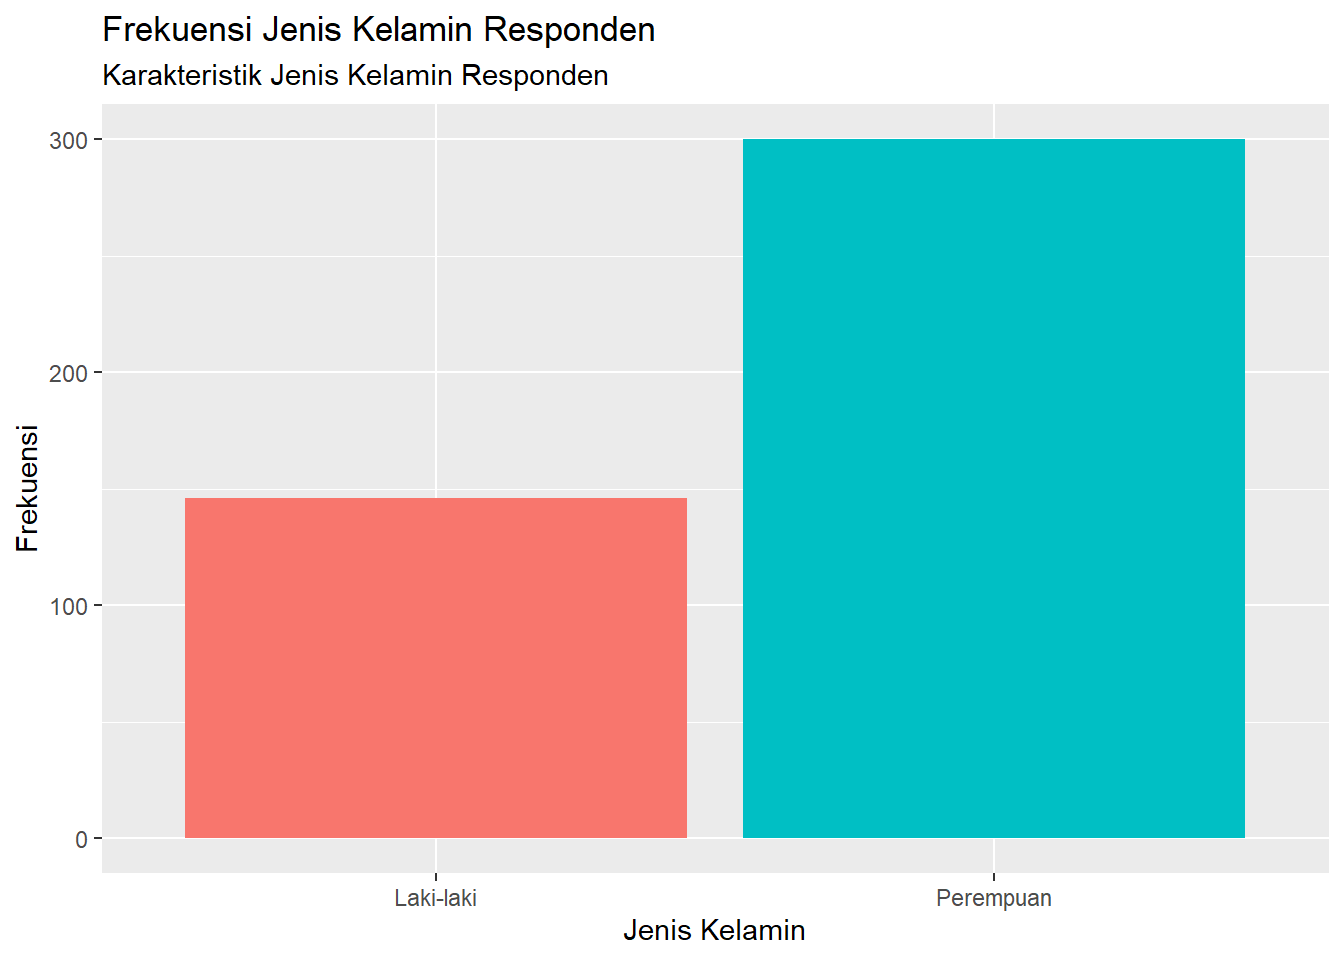
\includegraphics{internetaddiction_files/figure-latex/unnamed-chunk-2-1.pdf}

\begin{Shaded}
\begin{Highlighting}[]
\NormalTok{fakultas}
\end{Highlighting}
\end{Shaded}

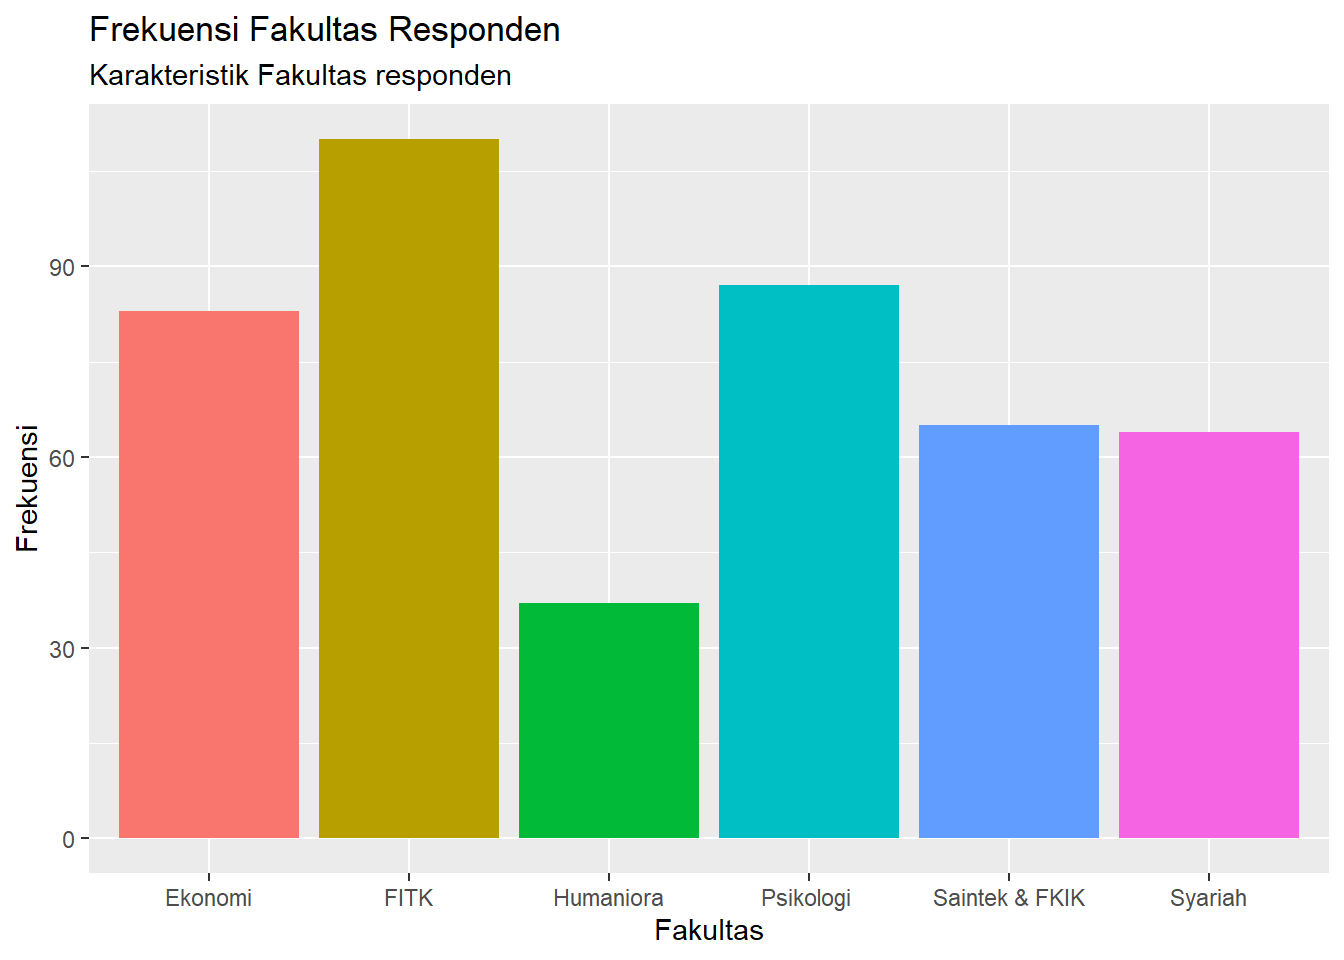
\includegraphics{internetaddiction_files/figure-latex/unnamed-chunk-2-2.pdf}

\textbf{\emph{Catatan}}

\begin{itemize}
\tightlist
\item
  Sebaran responden menurut jenis kelamin adalah ``Laki-laki'' sebanyak
  146 orang dan ``Perempuan'' 300 orang
\item
  Untuk sebaran fakultas: Ekonimi = 83 orang, FITK = 110 orang,
  Humaniora = 37 orang, Psikologi 87 orang, Saintek = 65 orang, dan
  Syariah = 64 orang
\end{itemize}

\hypertarget{menyederhanakan-variabel-jenis-kelamin-dan-fakultas}{%
\subsection{\texorpdfstring{\emph{Menyederhanakan Variabel Jenis Kelamin
dan
Fakultas}}{Menyederhanakan Variabel Jenis Kelamin dan Fakultas}}\label{menyederhanakan-variabel-jenis-kelamin-dan-fakultas}}

Dua visualisasi di atas dapat disederhanakan menjadi satu chart dengan
cara mengisi chartnya dengan variabel lain

\begin{Shaded}
\begin{Highlighting}[]
\CommentTok{# c) Menggabungkan variabel Sex dan Fakultas dalam satu chart (fill =) }
\NormalTok{internetdata }\OperatorTok
\StringTok{  }\KeywordTok{ggplot}\NormalTok{(}\KeywordTok{aes}\NormalTok{(}\DataTypeTok{x =}\NormalTok{ Fakultas, }\DataTypeTok{fill =}\NormalTok{ Sex)) }\OperatorTok{+}
\StringTok{  }\KeywordTok{geom_bar}\NormalTok{(}\DataTypeTok{alpha =} \DecValTok{3}\OperatorTok{/}\DecValTok{5}\NormalTok{) }\OperatorTok{+}
\StringTok{  }\KeywordTok{labs}\NormalTok{(}\DataTypeTok{title =} \StringTok{"Karakteristik Fakultas Responden"}\NormalTok{,}
  \DataTypeTok{subtitle =} \StringTok{"Dipecah dari Jenis Kelamin"}\NormalTok{,}
       \DataTypeTok{y =} \StringTok{"Frekuensi"}\NormalTok{, }
       \DataTypeTok{x =} \StringTok{"Fakultas"}\NormalTok{)}
\end{Highlighting}
\end{Shaded}

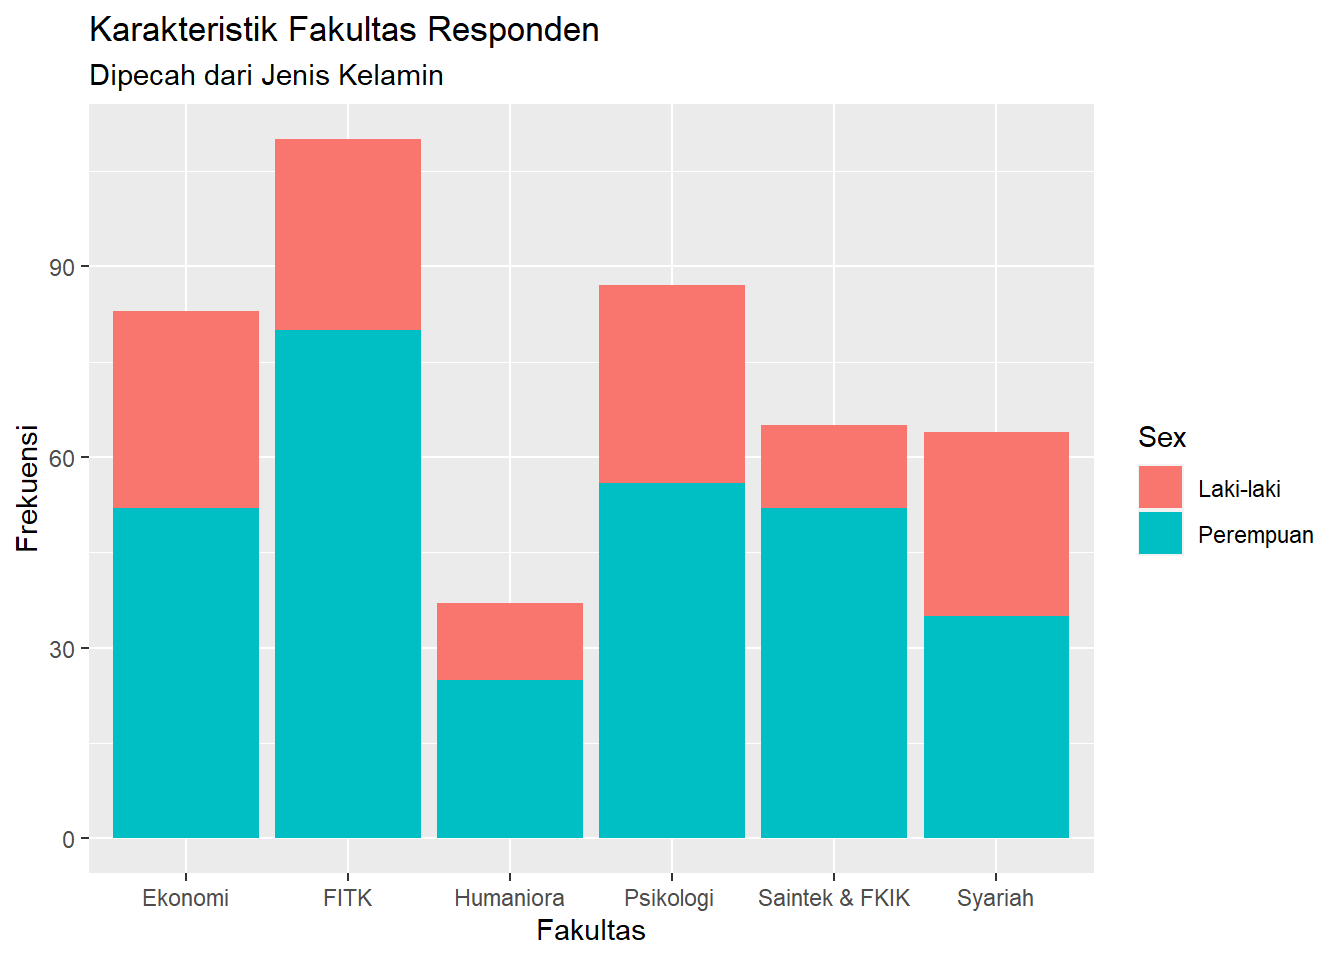
\includegraphics{internetaddiction_files/figure-latex/unnamed-chunk-3-1.pdf}

\textbf{\emph{Catatan}}

\begin{itemize}
\tightlist
\item
  Alih-alih memisahkan dua kategori demografi Fakultas dan Sex, akan
  lebih sederhana jika disatukan dengan hasil yang sama
\end{itemize}

\hypertarget{menggunakan-facet-wrap-untuk-menjabarkan-data}{%
\subsection{\texorpdfstring{\emph{Menggunakan Facet Wrap untuk
Menjabarkan
Data}}{Menggunakan Facet Wrap untuk Menjabarkan Data}}\label{menggunakan-facet-wrap-untuk-menjabarkan-data}}

Kita juga dapat membuat visualisasi dengan facet\_wrap untuk melihat
lebih detail bagaimana karakteristik jenis kelamin dan fakultas dipecah
menggunakan data koneksi

\begin{Shaded}
\begin{Highlighting}[]
\CommentTok{# d) Mem-facet_wrap menggunakan variabel Koneksi}
\NormalTok{internetdata }\OperatorTok
\StringTok{  }\KeywordTok{ggplot}\NormalTok{(}\KeywordTok{aes}\NormalTok{(}\DataTypeTok{x =}\NormalTok{ Koneksi, }\DataTypeTok{fill =}\NormalTok{ Sex)) }\OperatorTok{+}
\StringTok{  }\KeywordTok{theme_bw}\NormalTok{() }\OperatorTok{+}
\StringTok{  }\KeywordTok{facet_wrap}\NormalTok{(}\OperatorTok{~}\StringTok{ }\NormalTok{Fakultas) }\OperatorTok{+}
\StringTok{  }\KeywordTok{geom_bar}\NormalTok{(}\DataTypeTok{alpha =} \DecValTok{3}\OperatorTok{/}\DecValTok{5}\NormalTok{) }\OperatorTok{+}
\StringTok{  }\KeywordTok{labs}\NormalTok{(}\DataTypeTok{title =} \StringTok{"Frekuensi Pengguna Paket Data dan WiFi"}\NormalTok{,}
       \DataTypeTok{subtitle =} \StringTok{"dari Masing-Masing Fakultas Menurut Jenis Kelamin"}\NormalTok{,}
       \DataTypeTok{x =} \StringTok{"Fakultas"}\NormalTok{, }
       \DataTypeTok{y =} \StringTok{"Frekuensi"}\NormalTok{)}
\end{Highlighting}
\end{Shaded}

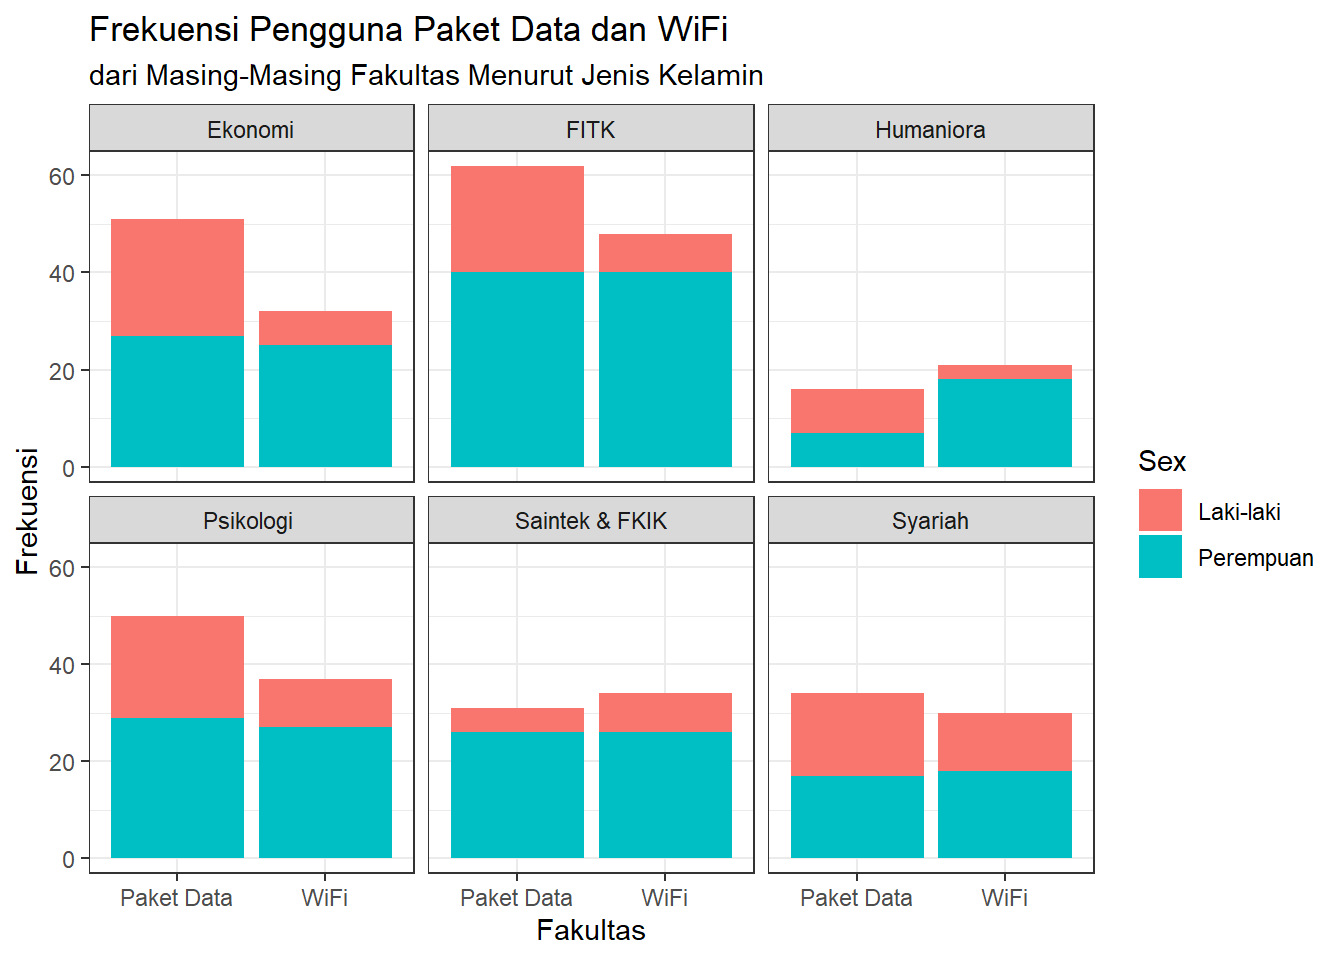
\includegraphics{internetaddiction_files/figure-latex/unnamed-chunk-4-1.pdf}

\textbf{\emph{Catatan}}

\begin{itemize}
\tightlist
\item
  Kita tidak bisa mentah-mentah menginterpretasikan data ini (i.e,
  pengguna paket data terbanyak dari FITK) karena jumlah responden per
  Fakultas yang tidak proporsional
\end{itemize}

\hypertarget{membuat-visualisasi-dari-variabel-medsos-media-sosial-yang-sering-digunakan-responden}{%
\subsection{\texorpdfstring{\emph{Membuat visualisasi dari variabel
MedSos (Media sosial yang sering digunakan
responden)}}{Membuat visualisasi dari variabel MedSos (Media sosial yang sering digunakan responden)}}\label{membuat-visualisasi-dari-variabel-medsos-media-sosial-yang-sering-digunakan-responden}}

Variabel MedSos menanyakan tentang jenis media sosial yang paling sering
digunakan oleh responden.

\begin{itemize}
\tightlist
\item
  Peneliti menyediakan beberapa jawaban media sosial serta menyertakan
  kolom kosong untuk diisi responden
\end{itemize}

\begin{Shaded}
\begin{Highlighting}[]
\NormalTok{treemap_medsos <-}\StringTok{ }\NormalTok{internetdata }\OperatorTok\StringTok{ }\KeywordTok{count}\NormalTok{(MedSos)}
\CommentTok{#View(treemap_medsos) # untuk melihat lebih detail tentang data }

\NormalTok{treemap_medsos }\OperatorTok\StringTok{ }
\StringTok{  }\KeywordTok{ggplot}\NormalTok{(}\KeywordTok{aes}\NormalTok{(}\DataTypeTok{fill =}\NormalTok{ MedSos,}
             \DataTypeTok{area =}\NormalTok{ n,}
             \DataTypeTok{label =}\NormalTok{ MedSos)) }\OperatorTok{+}
\StringTok{  }\KeywordTok{geom_treemap}\NormalTok{() }\OperatorTok{+}
\StringTok{  }\KeywordTok{geom_treemap_text}\NormalTok{(}\DataTypeTok{colour =} \StringTok{"white"}\NormalTok{,}
                    \DataTypeTok{place =} \StringTok{"centre"}\NormalTok{) }\OperatorTok{+}
\StringTok{  }\KeywordTok{labs}\NormalTok{(}\StringTok{"Media Sosial yang Sering Digunkan"}\NormalTok{) }\OperatorTok{+}
\StringTok{  }\KeywordTok{theme}\NormalTok{(}\DataTypeTok{legend.position =} \StringTok{"none"}\NormalTok{)}
\end{Highlighting}
\end{Shaded}

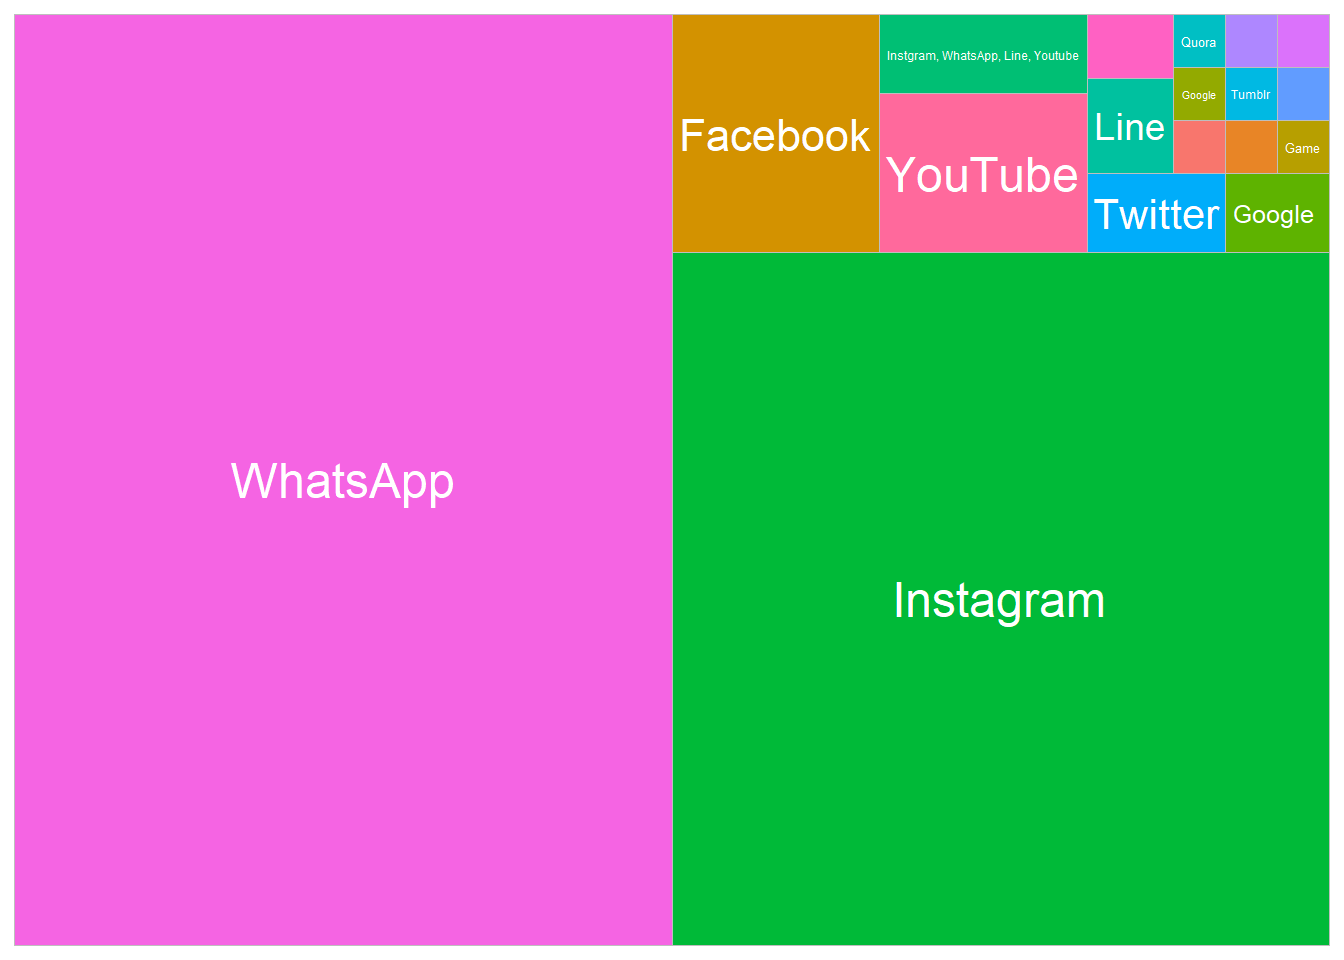
\includegraphics{internetaddiction_files/figure-latex/unnamed-chunk-5-1.pdf}

\textbf{\emph{Catatan}}

\begin{itemize}
\tightlist
\item
  Visualisasi di atas menunjukkan bahwa mayoritas responden mengaku
  lebih sering menggunakan media sosial WhatsApp (223 orang)
\item
  Mayoritas responden (166 orang) mengaku lebih sering menggunakan media
  sosial Instagram
\end{itemize}

\hypertarget{membuat-visualisasi-dari-variabel-alasan-alasan-responden-menggunakan-internet}{%
\subsection{\texorpdfstring{\emph{Membuat visualisasi dari variabel
Alasan (Alasan responden menggunakan
internet)}}{Membuat visualisasi dari variabel Alasan (Alasan responden menggunakan internet)}}\label{membuat-visualisasi-dari-variabel-alasan-alasan-responden-menggunakan-internet}}

Variabel Alasan mencoba untuk mengetahui alasan di balik akses internet
para responden. Hal ini memungkinkan untuk * Peneliti telah menyediakan
4 jawaban untuk dipilih responden

\begin{Shaded}
\begin{Highlighting}[]
\NormalTok{treemap_alasan <-}\StringTok{ }\NormalTok{internetdata }\OperatorTok\StringTok{ }\KeywordTok{count}\NormalTok{(Alasan)}
  
\NormalTok{treemap_alasan }\OperatorTok\StringTok{ }\KeywordTok{ggplot}\NormalTok{(}\KeywordTok{aes}\NormalTok{(}\DataTypeTok{fill =}\NormalTok{ Alasan, }
                            \DataTypeTok{area =}\NormalTok{ n,}
                            \DataTypeTok{label =}\NormalTok{ Alasan)) }\OperatorTok{+}
\StringTok{  }\KeywordTok{geom_treemap}\NormalTok{() }\OperatorTok{+}
\StringTok{  }\KeywordTok{geom_treemap_text}\NormalTok{(}\DataTypeTok{colour =} \StringTok{"white"}\NormalTok{,}
                    \DataTypeTok{place =} \StringTok{"centre"}\NormalTok{) }\OperatorTok{+}
\StringTok{  }\KeywordTok{labs}\NormalTok{(}\StringTok{"Alasan Penggunaan Internet"}\NormalTok{) }\OperatorTok{+}
\StringTok{  }\KeywordTok{theme}\NormalTok{(}\DataTypeTok{legend.position =} \StringTok{"none"}\NormalTok{)}
\end{Highlighting}
\end{Shaded}

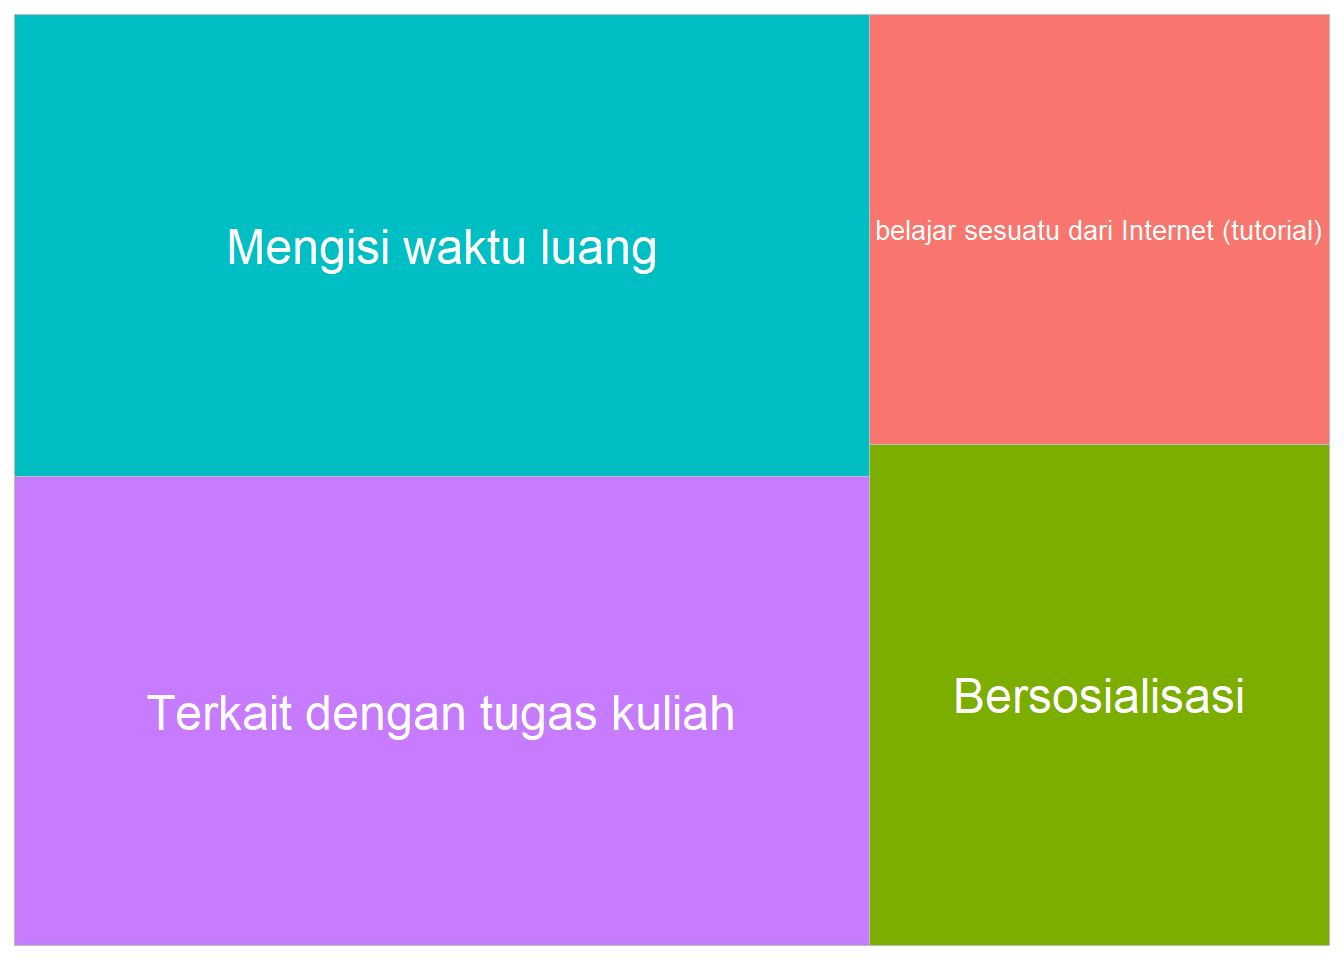
\includegraphics{internetaddiction_files/figure-latex/unnamed-chunk-6-1.pdf}

\textbf{\emph{Catatan}}

\begin{itemize}
\tightlist
\item
  Visualisasi treemap di atas menunjukkan bahwa mayoritas responden
  cenderung menggunakan internet karena terkait tugas kuliah dan mengisi
  waktu luang
\end{itemize}

\hypertarget{bagaimana-tentang-usia-responden}{%
\subsection{\texorpdfstring{\emph{Bagaimana tentang usia
responden?}}{Bagaimana tentang usia responden?}}\label{bagaimana-tentang-usia-responden}}

\begin{Shaded}
\begin{Highlighting}[]
\NormalTok{internetdata }\OperatorTok\StringTok{ }\KeywordTok{ggplot}\NormalTok{(}\KeywordTok{aes}\NormalTok{(}\DataTypeTok{x =}\NormalTok{ Usia)) }\OperatorTok{+}
\StringTok{  }\KeywordTok{geom_histogram}\NormalTok{(}\DataTypeTok{binwidth =} \DecValTok{1}\NormalTok{,  }\DataTypeTok{fill =} \StringTok{"deepskyblue3"}\NormalTok{) }\OperatorTok{+}\StringTok{ }
\StringTok{  }\KeywordTok{labs}\NormalTok{(}\DataTypeTok{y =} \StringTok{"Jumlah Responden"}\NormalTok{, }
       \DataTypeTok{x =} \StringTok{"Usia (binwidth = 1)"}\NormalTok{,}
       \DataTypeTok{title =} \StringTok{"Internet Addiction Responden Age Distribution"}\NormalTok{)}
\end{Highlighting}
\end{Shaded}

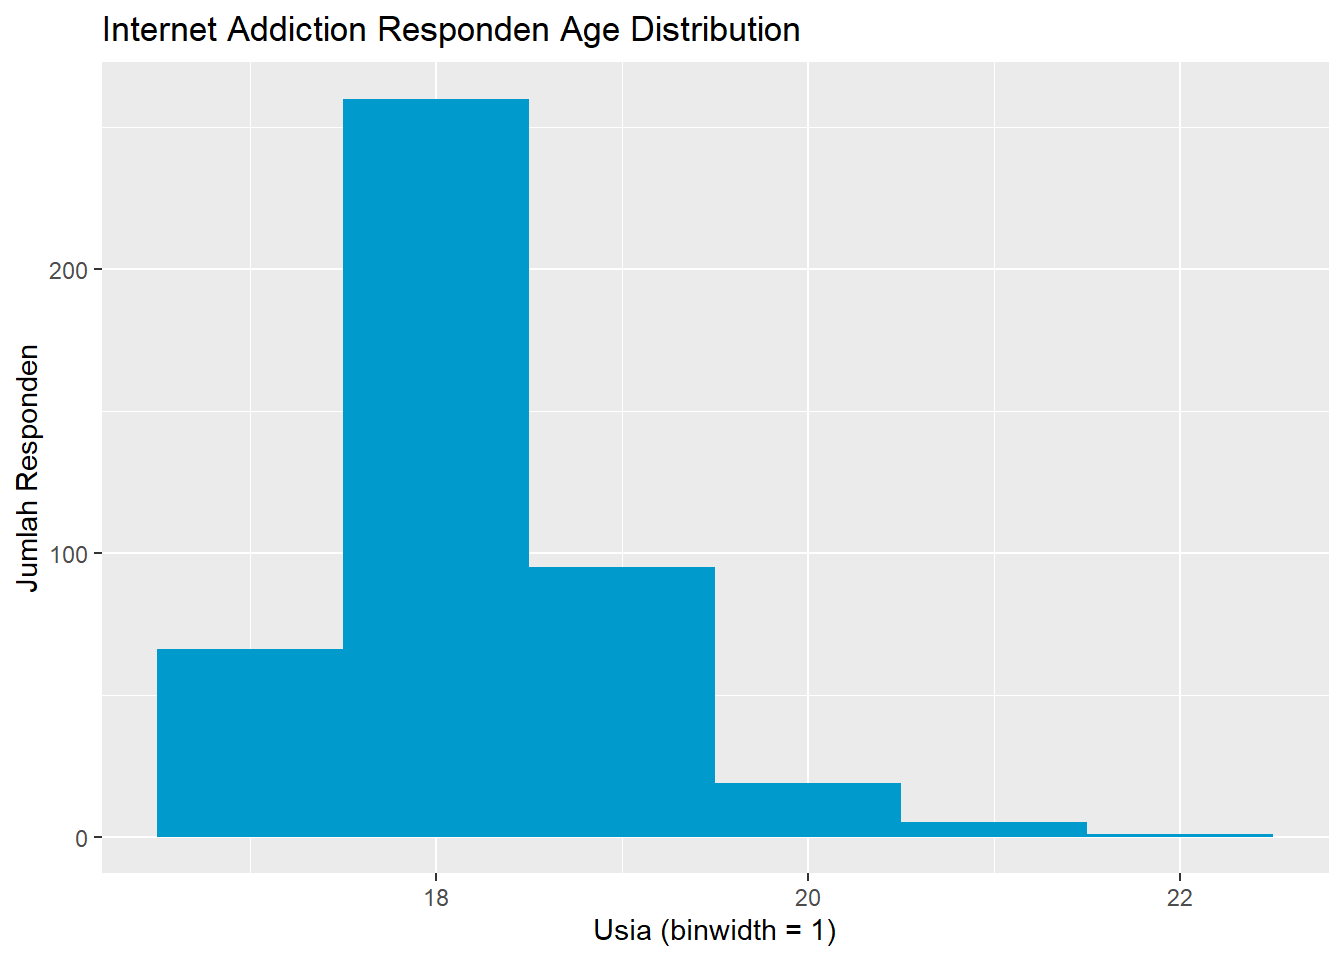
\includegraphics{internetaddiction_files/figure-latex/unnamed-chunk-7-1.pdf}

\textbf{\emph{Catatan}}

\begin{itemize}
\tightlist
\item
  Mayoritas responden berada pada usia 18 tahun (260 orang)
\item
  Hanya 5 orang yang berusia 21 tahun dan 1 orang berusia 22 tahun
\end{itemize}

\hypertarget{visualisasi-dan-analisa-variabel-kategori-adiksi}{%
\section{\texorpdfstring{\textbf{Visualisasi dan Analisa Variabel
Kategori
Adiksi}}{Visualisasi dan Analisa Variabel Kategori Adiksi}}\label{visualisasi-dan-analisa-variabel-kategori-adiksi}}

\hypertarget{membuat-visualisasi-dari-variabel-kategori}{%
\subsection{\texorpdfstring{\emph{Membuat visualisasi dari variabel
``Kategori''}}{Membuat visualisasi dari variabel ``Kategori''}}\label{membuat-visualisasi-dari-variabel-kategori}}

\begin{Shaded}
\begin{Highlighting}[]
\NormalTok{kategori <-}\StringTok{ }\NormalTok{internetdata }\OperatorTok\StringTok{ }
\StringTok{  }\KeywordTok{ggplot}\NormalTok{(}\KeywordTok{aes}\NormalTok{(}\DataTypeTok{x =}\NormalTok{ Kategori, }
             \DataTypeTok{fill =}\NormalTok{ Kategori)) }\OperatorTok{+}
\StringTok{  }\KeywordTok{geom_bar}\NormalTok{(}\DataTypeTok{alpha =} \DecValTok{3}\OperatorTok{/}\DecValTok{5}\NormalTok{) }\OperatorTok{+}
\StringTok{  }\KeywordTok{labs}\NormalTok{(}\DataTypeTok{title =} \StringTok{"Responden dengan Kategori Adiksi dan Nonadiksi"}\NormalTok{,}
       \DataTypeTok{x =} \StringTok{"Kategori"}\NormalTok{, }
       \DataTypeTok{y =} \StringTok{"Frekuensi"}\NormalTok{) }\OperatorTok{+}
\StringTok{  }\KeywordTok{theme}\NormalTok{(}\DataTypeTok{legend.position =} \StringTok{"none"}\NormalTok{)}

\NormalTok{kategori}
\end{Highlighting}
\end{Shaded}

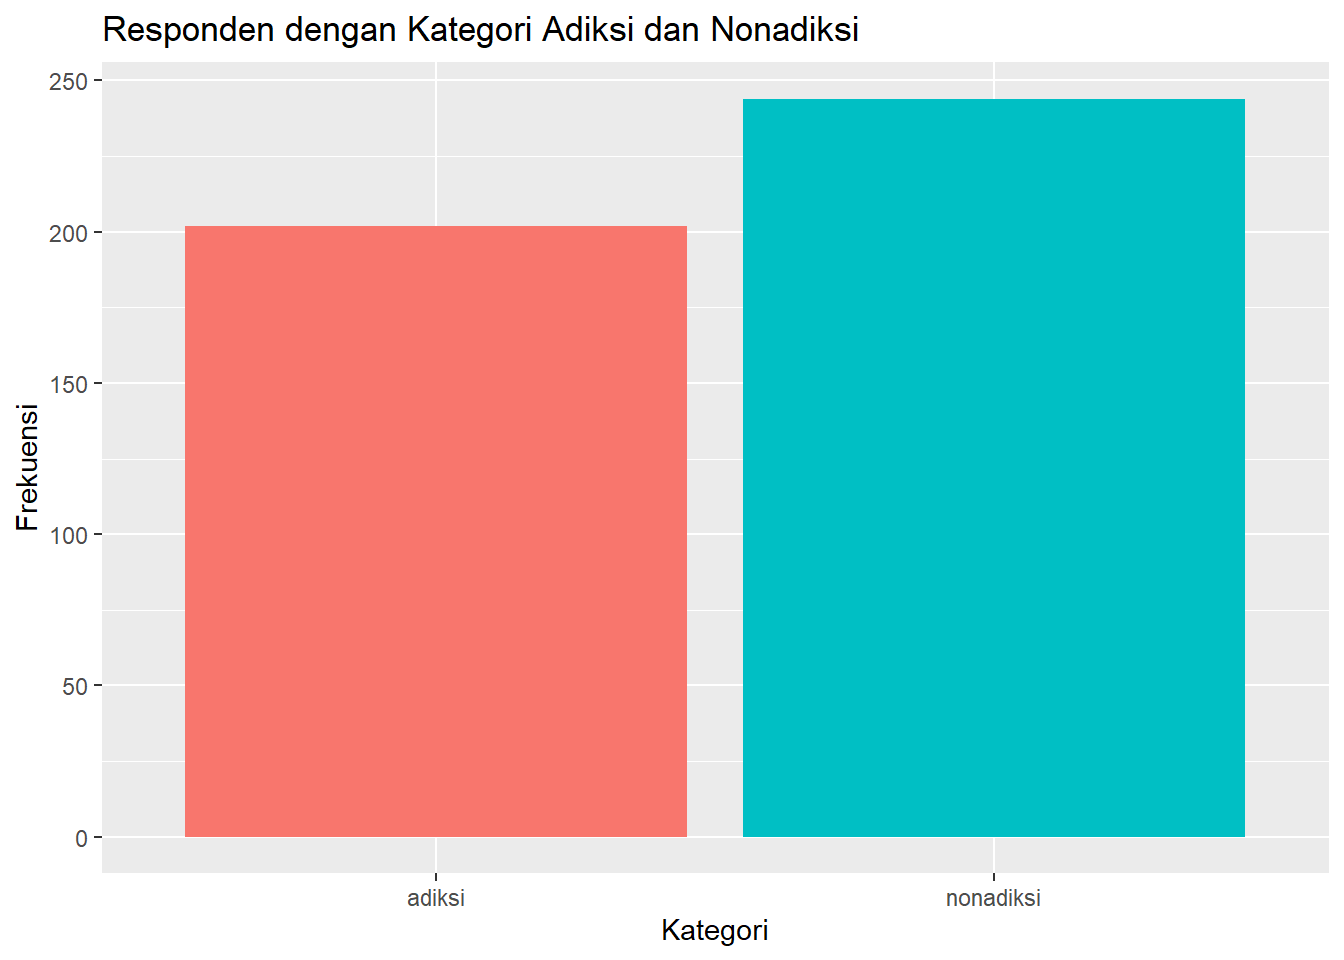
\includegraphics{internetaddiction_files/figure-latex/unnamed-chunk-8-1.pdf}

\begin{Shaded}
\begin{Highlighting}[]
\KeywordTok{prop.table}\NormalTok{(}\KeywordTok{table}\NormalTok{(internetdata}\OperatorTok{$}\NormalTok{Kategori))}
\end{Highlighting}
\end{Shaded}

\begin{verbatim}
## 
##    adiksi nonadiksi 
## 0.4529148 0.5470852
\end{verbatim}

\textbf{\emph{Catatan}}

\begin{itemize}
\item
  Sebanyak 218 orang (49 persen) termasuk dalam kategori adiksi
  sedangkan 228 orang lainnya (51 persen) berada dalam kategori
  nonadiksi
\item
  Untuk mengingatkan bahwa variabel kategori diambil dari angka mean
  variabel IA
\end{itemize}

\hypertarget{kategori-kecanduan-berdasarkan-jenis-kelamin-dan-usia}{%
\subsection{\texorpdfstring{\emph{Kategori Kecanduan Berdasarkan Jenis
Kelamin dan
Usia}}{Kategori Kecanduan Berdasarkan Jenis Kelamin dan Usia}}\label{kategori-kecanduan-berdasarkan-jenis-kelamin-dan-usia}}

\begin{Shaded}
\begin{Highlighting}[]
\NormalTok{kategori_sex <-}\StringTok{ }\NormalTok{internetdata }\OperatorTok\StringTok{ }
\StringTok{  }\KeywordTok{ggplot}\NormalTok{(}\KeywordTok{aes}\NormalTok{(}\DataTypeTok{x =}\NormalTok{ Sex, }\DataTypeTok{fill =}\NormalTok{ Kategori)) }\OperatorTok{+}
\StringTok{  }\KeywordTok{theme_bw}\NormalTok{() }\OperatorTok{+}\StringTok{ }
\StringTok{  }\KeywordTok{geom_bar}\NormalTok{() }\OperatorTok{+}\StringTok{ }
\StringTok{  }\KeywordTok{labs}\NormalTok{(}\DataTypeTok{y =} \StringTok{"Frekuensi Responden"}\NormalTok{, }
       \DataTypeTok{title =} \StringTok{"Frekuensi Kategori dari Gender"}\NormalTok{)}

\NormalTok{kategori_usia <-}\StringTok{ }\NormalTok{internetdata }\OperatorTok\StringTok{ }
\StringTok{  }\KeywordTok{ggplot}\NormalTok{(}\KeywordTok{aes}\NormalTok{(}\DataTypeTok{x =}\NormalTok{ Usia, }\DataTypeTok{fill =}\NormalTok{ Kategori)) }\OperatorTok{+}
\StringTok{  }\KeywordTok{theme_bw}\NormalTok{() }\OperatorTok{+}
\StringTok{  }\KeywordTok{geom_bar}\NormalTok{() }\OperatorTok{+}
\StringTok{  }\KeywordTok{labs}\NormalTok{(}\DataTypeTok{y =} \StringTok{"Frekuensi Responden"}\NormalTok{, }
       \DataTypeTok{title =} \StringTok{"Frekuensi Kategori dari Usia"}\NormalTok{)}


\NormalTok{kategori_sex}
\end{Highlighting}
\end{Shaded}

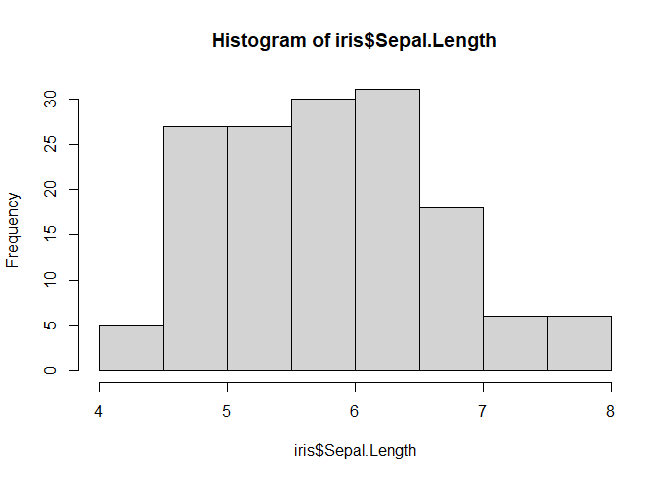
\includegraphics{internetaddiction_files/figure-latex/unnamed-chunk-9-1.pdf}

\begin{Shaded}
\begin{Highlighting}[]
\NormalTok{kategori_usia}
\end{Highlighting}
\end{Shaded}

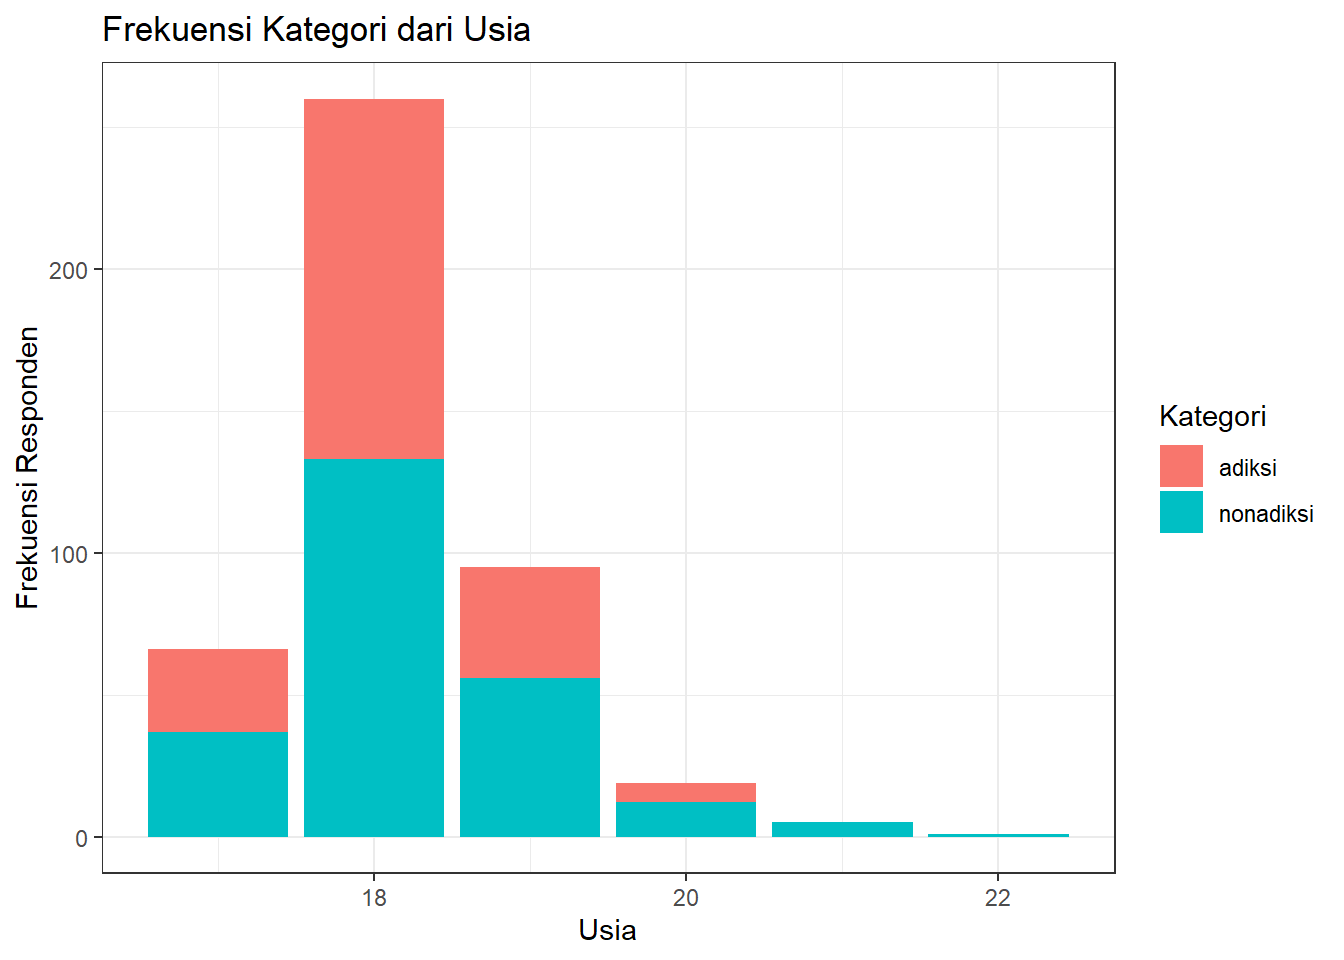
\includegraphics{internetaddiction_files/figure-latex/unnamed-chunk-9-2.pdf}

\textbf{\emph{Catatan}}

\begin{itemize}
\tightlist
\item
  Dari jenis kelamin laki-laki 84 orang termasuk dalam kategori adiksi
  dan 62 orang termasuk dalam kategori nonadiksi. Sedang untuk
  perempuan, sebanyak 134 orang termasuk dalam kategori adiksi dan 166
  orang termasuk dalam kategori nonadiksi
\end{itemize}

\hypertarget{facet-wrap-koneksi-dari-jenis-kelamin-diisi-dengan-variabel-kategori}{%
\subsection{\texorpdfstring{\emph{Facet-Wrap Koneksi dari Jenis Kelamin
Diisi dengan Variabel
``Kategori''}}{Facet-Wrap Koneksi dari Jenis Kelamin Diisi dengan Variabel ``Kategori''}}\label{facet-wrap-koneksi-dari-jenis-kelamin-diisi-dengan-variabel-kategori}}

\begin{Shaded}
\begin{Highlighting}[]
\NormalTok{internetdata }\OperatorTok\StringTok{ }
\StringTok{  }\KeywordTok{ggplot}\NormalTok{(}\KeywordTok{aes}\NormalTok{(}\DataTypeTok{x =}\NormalTok{ Sex, }\DataTypeTok{fill =}\NormalTok{ Kategori)) }\OperatorTok{+}
\StringTok{  }\KeywordTok{theme_bw}\NormalTok{() }\OperatorTok{+}
\StringTok{  }\KeywordTok{facet_wrap}\NormalTok{(}\OperatorTok{~}\StringTok{ }\NormalTok{Koneksi) }\OperatorTok{+}
\StringTok{  }\KeywordTok{geom_bar}\NormalTok{() }\OperatorTok{+}\StringTok{ }
\StringTok{  }\KeywordTok{labs}\NormalTok{(}\DataTypeTok{y =} \StringTok{"Frekuensi Responden"}\NormalTok{, }
       \DataTypeTok{title =} \StringTok{"Variabel Jenis Kelamin dari Koneksi yang Digunakan"}\NormalTok{)}
\end{Highlighting}
\end{Shaded}

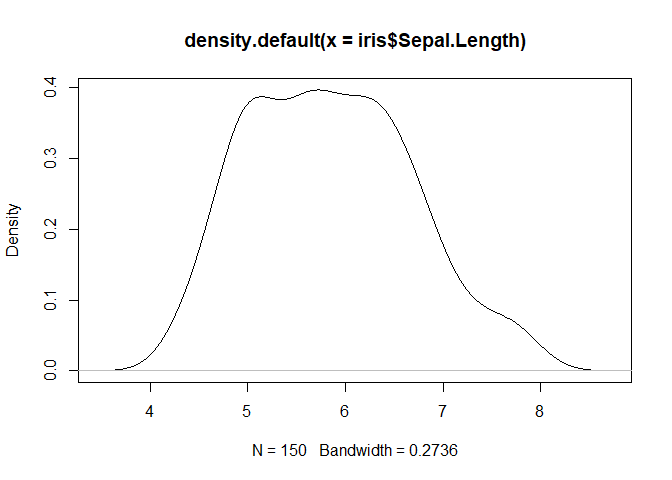
\includegraphics{internetaddiction_files/figure-latex/unnamed-chunk-10-1.pdf}

\hypertarget{menghubungkan-variabel-kategori-jenis-kelamin-dan-koneksi}{%
\subsection{\texorpdfstring{\emph{Menghubungkan variabel kategori, jenis
kelamin dan
koneksi}}{Menghubungkan variabel kategori, jenis kelamin dan koneksi}}\label{menghubungkan-variabel-kategori-jenis-kelamin-dan-koneksi}}

\begin{Shaded}
\begin{Highlighting}[]
\NormalTok{internetall <-}\StringTok{ }\NormalTok{internetdata }\OperatorTok
\StringTok{  }\KeywordTok{group_by}\NormalTok{(Kategori, Sex, Koneksi) }\OperatorTok
\StringTok{  }\KeywordTok{count}\NormalTok{()}

\NormalTok{konekallu <-}\StringTok{ }\KeywordTok{ggplot}\NormalTok{(internetall, }
       \KeywordTok{aes}\NormalTok{(}\DataTypeTok{axis1 =}\NormalTok{ Koneksi,}
           \DataTypeTok{axis2 =}\NormalTok{ Kategori,}
           \DataTypeTok{y =}\NormalTok{ n)) }\OperatorTok{+}
\StringTok{  }\KeywordTok{geom_alluvium}\NormalTok{(}\KeywordTok{aes}\NormalTok{(}\DataTypeTok{fill =}\NormalTok{ Sex)) }\OperatorTok{+}
\StringTok{  }\KeywordTok{geom_stratum}\NormalTok{() }\OperatorTok{+}
\StringTok{  }\KeywordTok{geom_text}\NormalTok{(}\DataTypeTok{stat =} \StringTok{"stratum"}\NormalTok{,}
            \KeywordTok{aes}\NormalTok{(}\DataTypeTok{label =} \KeywordTok{after_stat}\NormalTok{(stratum))) }\OperatorTok{+}
\StringTok{  }\KeywordTok{scale_x_discrete}\NormalTok{(}\DataTypeTok{limits =} \KeywordTok{c}\NormalTok{(}\StringTok{"Koneksi"}\NormalTok{, }\StringTok{"Kategori"}\NormalTok{),}
                   \DataTypeTok{expand =} \KeywordTok{c}\NormalTok{(.}\DecValTok{1}\NormalTok{, }\FloatTok{.1}\NormalTok{)) }\OperatorTok{+}
\StringTok{  }\KeywordTok{labs}\NormalTok{(}\DataTypeTok{title =} \StringTok{"Internet Data"}\NormalTok{,}
       \DataTypeTok{subtitle =} \StringTok{"stratified by koneksi, sex, and kategori"}\NormalTok{,}
       \DataTypeTok{y =} \StringTok{"Frequency"}\NormalTok{) }\OperatorTok{+}
\StringTok{  }\KeywordTok{theme_minimal}\NormalTok{()}



\NormalTok{durasiAllu <-}\StringTok{ }\NormalTok{internetdata }\OperatorTok
\StringTok{  }\KeywordTok{group_by}\NormalTok{(Durasi, Sex, Kategori) }\OperatorTok
\StringTok{  }\KeywordTok{count}\NormalTok{()}

\NormalTok{duraAlu <-}\StringTok{ }\KeywordTok{ggplot}\NormalTok{(durasiAllu, }
       \KeywordTok{aes}\NormalTok{(}\DataTypeTok{axis1 =}\NormalTok{ Durasi,}
           \DataTypeTok{axis2 =}\NormalTok{ Kategori,}
           \DataTypeTok{y =}\NormalTok{ n)) }\OperatorTok{+}
\StringTok{  }\KeywordTok{geom_alluvium}\NormalTok{(}\KeywordTok{aes}\NormalTok{(}\DataTypeTok{fill =}\NormalTok{ Sex)) }\OperatorTok{+}
\StringTok{  }\KeywordTok{geom_stratum}\NormalTok{() }\OperatorTok{+}
\StringTok{  }\KeywordTok{geom_text}\NormalTok{(}\DataTypeTok{stat =} \StringTok{"stratum"}\NormalTok{,}
            \KeywordTok{aes}\NormalTok{(}\DataTypeTok{label =} \KeywordTok{after_stat}\NormalTok{(stratum))) }\OperatorTok{+}
\StringTok{  }\KeywordTok{scale_x_discrete}\NormalTok{(}\DataTypeTok{limits =} \KeywordTok{c}\NormalTok{(}\StringTok{"Durasi"}\NormalTok{, }\StringTok{"Kategori"}\NormalTok{),}
                   \DataTypeTok{expand =} \KeywordTok{c}\NormalTok{(.}\DecValTok{1}\NormalTok{, }\FloatTok{.1}\NormalTok{)) }\OperatorTok{+}
\StringTok{  }\KeywordTok{labs}\NormalTok{(}\DataTypeTok{title =} \StringTok{"Internet Data"}\NormalTok{,}
       \DataTypeTok{subtitle =} \StringTok{"stratified by durasi, sex, and kategori"}\NormalTok{,}
       \DataTypeTok{y =} \StringTok{"Frequency"}\NormalTok{) }\OperatorTok{+}
\StringTok{  }\KeywordTok{theme_minimal}\NormalTok{()}


\NormalTok{konekallu}
\end{Highlighting}
\end{Shaded}

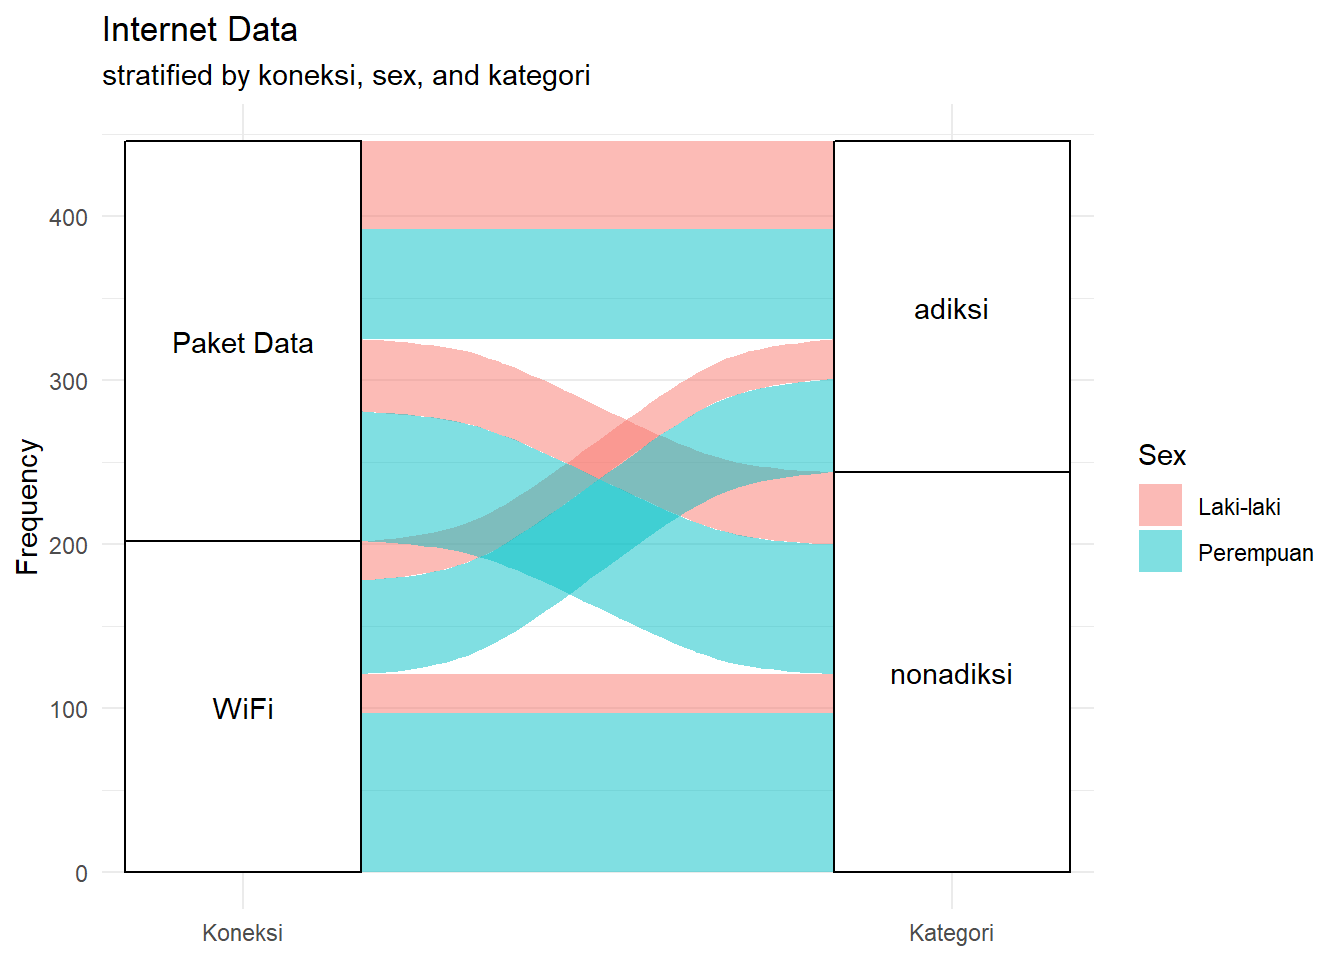
\includegraphics{internetaddiction_files/figure-latex/unnamed-chunk-11-1.pdf}

\begin{Shaded}
\begin{Highlighting}[]
\NormalTok{duraAlu}
\end{Highlighting}
\end{Shaded}

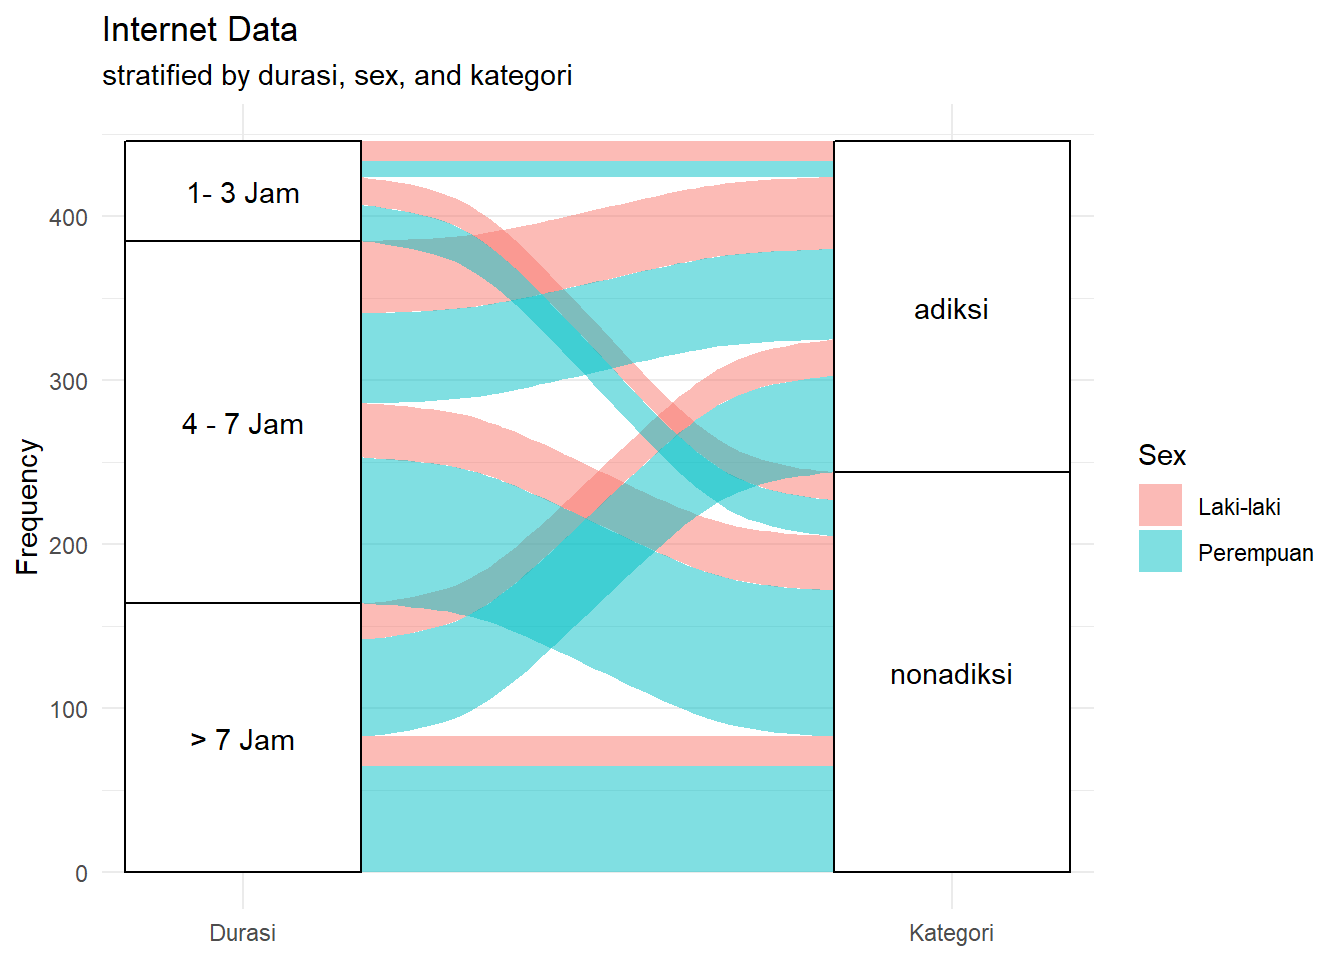
\includegraphics{internetaddiction_files/figure-latex/unnamed-chunk-11-2.pdf}

\hypertarget{membuat-diagram-alluvial-menggunakan-4-variabel}{%
\subsection{\texorpdfstring{\emph{Membuat diagram alluvial menggunakan 4
variabel}}{Membuat diagram alluvial menggunakan 4 variabel}}\label{membuat-diagram-alluvial-menggunakan-4-variabel}}

\begin{Shaded}
\begin{Highlighting}[]
\NormalTok{internetall2 <-}\StringTok{ }\NormalTok{internetdata }\OperatorTok\StringTok{ }
\StringTok{  }\KeywordTok{group_by}\NormalTok{(Kategori, Sex, Koneksi, Fakultas) }\OperatorTok
\StringTok{  }\KeywordTok{count}\NormalTok{()}

\KeywordTok{ggplot}\NormalTok{(internetall2, }
       \KeywordTok{aes}\NormalTok{(}\DataTypeTok{axis1 =}\NormalTok{ Kategori,}
           \DataTypeTok{axis2 =}\NormalTok{ Koneksi,}
           \DataTypeTok{axis3 =}\NormalTok{ Fakultas,}
           \DataTypeTok{y =}\NormalTok{ n)) }\OperatorTok{+}
\StringTok{  }\KeywordTok{geom_alluvium}\NormalTok{(}\KeywordTok{aes}\NormalTok{(}\DataTypeTok{fill =}\NormalTok{ Sex)) }\OperatorTok{+}
\StringTok{  }\KeywordTok{geom_stratum}\NormalTok{() }\OperatorTok{+}
\StringTok{  }\KeywordTok{geom_text}\NormalTok{(}\DataTypeTok{stat =} \StringTok{"stratum"}\NormalTok{, }
            \KeywordTok{aes}\NormalTok{(}\DataTypeTok{label =} \KeywordTok{after_stat}\NormalTok{(stratum))) }\OperatorTok{+}
\StringTok{  }\KeywordTok{scale_x_discrete}\NormalTok{(}\DataTypeTok{limits =} \KeywordTok{c}\NormalTok{(}\StringTok{"Kategori"}\NormalTok{, }\StringTok{"Koneksi"}\NormalTok{, }\StringTok{"Fakultas"}\NormalTok{),}
                   \DataTypeTok{expand =} \KeywordTok{c}\NormalTok{(.}\DecValTok{1}\NormalTok{, }\FloatTok{.1}\NormalTok{)) }\OperatorTok{+}
\StringTok{  }\KeywordTok{scale_fill_viridis_d}\NormalTok{() }\OperatorTok{+}
\StringTok{  }\KeywordTok{labs}\NormalTok{(}\DataTypeTok{title =} \StringTok{"Internet Data"}\NormalTok{,}
       \DataTypeTok{subtitle =} \StringTok{"stratified by addicting category, koneksi, dan layanan"}\NormalTok{,}
       \DataTypeTok{y =} \StringTok{"Frequency"}\NormalTok{,}
       \DataTypeTok{x =} \StringTok{"Demographic"}\NormalTok{) }\OperatorTok{+}
\StringTok{  }\KeywordTok{theme_minimal}\NormalTok{() }
\end{Highlighting}
\end{Shaded}

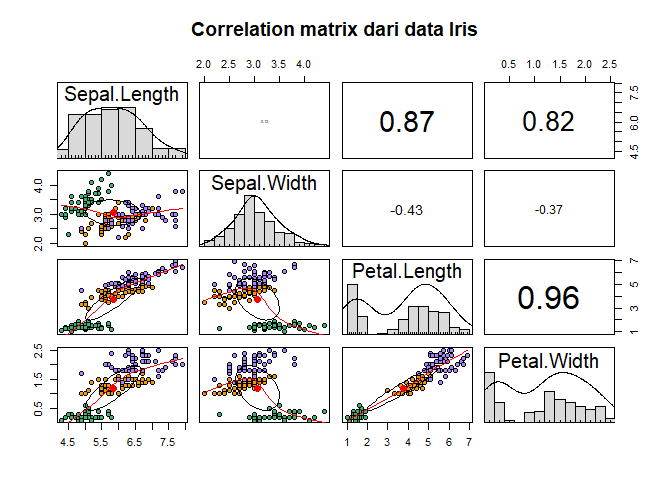
\includegraphics{internetaddiction_files/figure-latex/unnamed-chunk-12-1.pdf}

\hypertarget{melihat-gambaran-demografi-kategori-jenis-kelamin-dan-koneksi}{%
\subsection{\texorpdfstring{\emph{Melihat gambaran demografi Kategori,
Jenis Kelamin, dan
Koneksi}}{Melihat gambaran demografi Kategori, Jenis Kelamin, dan Koneksi}}\label{melihat-gambaran-demografi-kategori-jenis-kelamin-dan-koneksi}}

\begin{Shaded}
\begin{Highlighting}[]
\NormalTok{jj <-}\StringTok{ }\KeywordTok{xtabs}\NormalTok{(}\OperatorTok{~}\NormalTok{Kategori }\OperatorTok{+}\StringTok{ }\NormalTok{Sex }\OperatorTok{+}\StringTok{ }\NormalTok{Koneksi, internetdata)}

\CommentTok{# mosaic(jj, main = "Internet Data") #ini memunculkan layer dasar }

\KeywordTok{mosaic}\NormalTok{(jj, }
       \DataTypeTok{shade =}\NormalTok{ T,}
       \DataTypeTok{legend =}\NormalTok{ T,}
       \DataTypeTok{labeling_args =} \KeywordTok{list}\NormalTok{(}\DataTypeTok{set_vernames =} \KeywordTok{c}\NormalTok{(}\DataTypeTok{Sex =} \StringTok{"Gender"}\NormalTok{,}
                                             \DataTypeTok{Kategori =} \StringTok{"Kategori Adiksi"}\NormalTok{,}
                                             \DataTypeTok{Koneksi =} \StringTok{"Tipe Koneksi"}\NormalTok{)),}
       \DataTypeTok{set_labels =} \KeywordTok{list}\NormalTok{(}\DataTypeTok{Kategori =} \KeywordTok{c}\NormalTok{(}\StringTok{"Yes"}\NormalTok{, }\StringTok{"No"}\NormalTok{),}
                         \DataTypeTok{Sex =} \KeywordTok{c}\NormalTok{(}\StringTok{"Pria"}\NormalTok{, }\StringTok{"Wanita"}\NormalTok{),}
                         \DataTypeTok{Koneksi =} \KeywordTok{c}\NormalTok{(}\StringTok{"Data"}\NormalTok{, }\StringTok{"Wifi"}\NormalTok{)),}
       \DataTypeTok{main =} \StringTok{"Internet Data"}\NormalTok{)}
\end{Highlighting}
\end{Shaded}

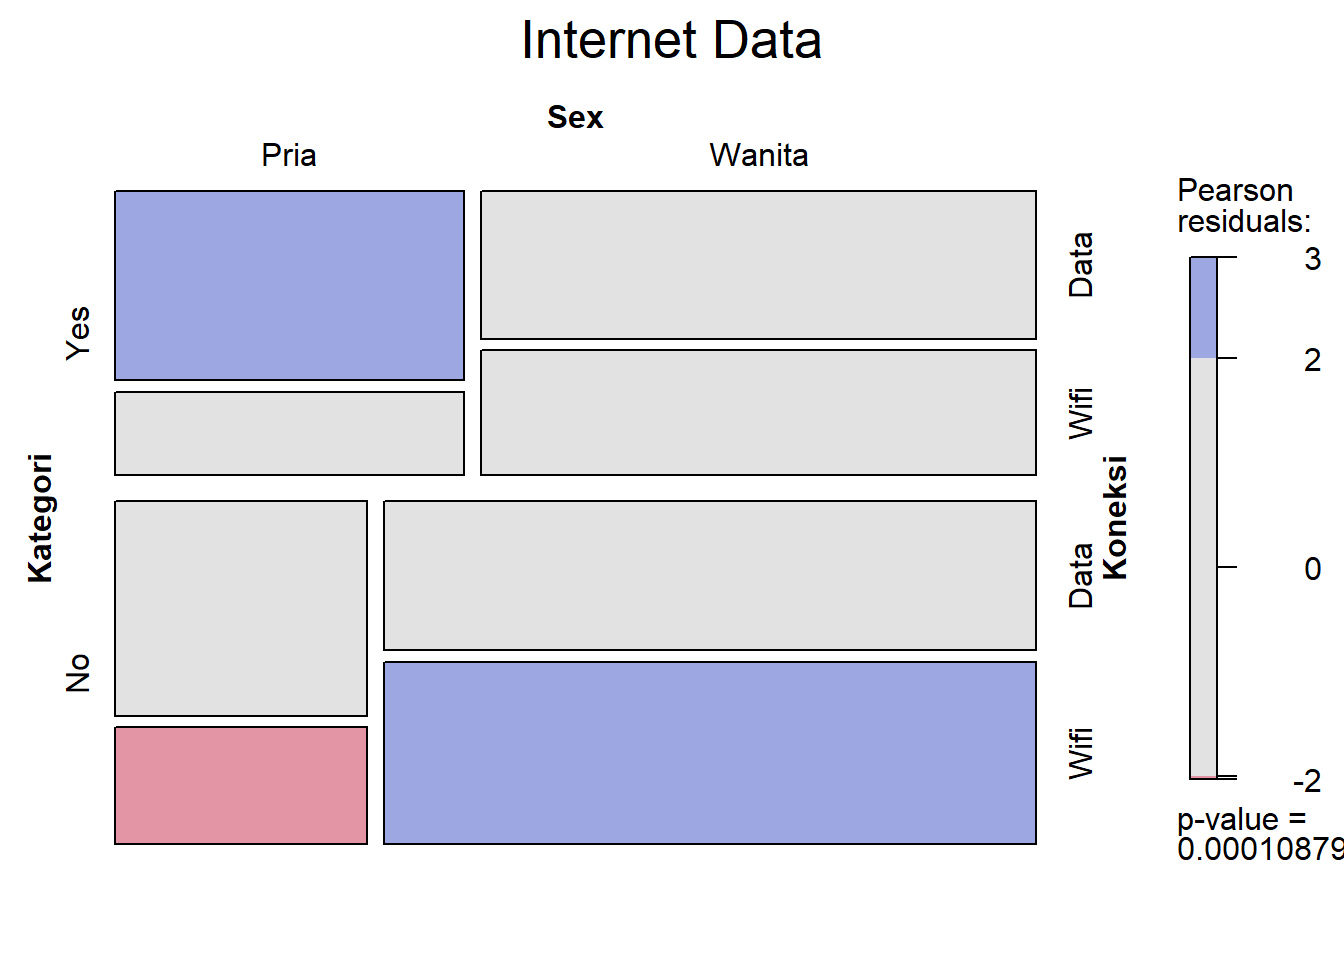
\includegraphics{internetaddiction_files/figure-latex/unnamed-chunk-13-1.pdf}

\hypertarget{analisis-statistik-dari-variabel-ia-depresi-anxiety-dan-stress}{%
\section{\texorpdfstring{\textbf{Analisis Statistik dari Variabel IA,
Depresi, Anxiety, dan
Stress}}{Analisis Statistik dari Variabel IA, Depresi, Anxiety, dan Stress}}\label{analisis-statistik-dari-variabel-ia-depresi-anxiety-dan-stress}}

Setelah dirasa cukup dengan data demografi, data dari variabel skala
psikologi juga harus dianalisis

4 variabel ini merupakan variabel utama dari penelitian

\hypertarget{summary-korelasi-4-variabel-psikologis}{%
\subsection{\texorpdfstring{\emph{Summary korelasi 4 variabel
psikologis}}{Summary korelasi 4 variabel psikologis}}\label{summary-korelasi-4-variabel-psikologis}}

Uji Statistik yang pertama dilakukan adalah dengan menemukan angka
korelasi dari empat variabel psikologis: Internet addiction, depresi,
anxiety, dan stress

\begin{Shaded}
\begin{Highlighting}[]
\CommentTok{#Menggunakan }
\CommentTok{#library(correlation)}

\NormalTok{newdata <-}\StringTok{ }\KeywordTok{select}\NormalTok{(internetdata, IA, Depresi, Anxiety, Stress)}
\NormalTok{correlation}\OperatorTok{::}\KeywordTok{correlation}\NormalTok{(newdata, }\DataTypeTok{include_factors =}\NormalTok{ T, }\DataTypeTok{method =} \StringTok{"auto"}\NormalTok{)}
\end{Highlighting}
\end{Shaded}

\begin{verbatim}
## Parameter1 | Parameter2 |    r |       95% CI |     t |  df |      p |  Method | n_Obs
## --------------------------------------------------------------------------------------
## IA         |    Depresi | 0.36 | [0.28, 0.44] |  8.14 | 444 | < .001 | Pearson |   446
## IA         |    Anxiety | 0.44 | [0.36, 0.51] | 10.20 | 444 | < .001 | Pearson |   446
## IA         |     Stress | 0.48 | [0.41, 0.55] | 11.59 | 444 | < .001 | Pearson |   446
## Depresi    |    Anxiety | 0.72 | [0.67, 0.76] | 21.68 | 444 | < .001 | Pearson |   446
## Depresi    |     Stress | 0.71 | [0.66, 0.75] | 21.24 | 444 | < .001 | Pearson |   446
## Anxiety    |     Stress | 0.79 | [0.75, 0.82] | 27.31 | 444 | < .001 | Pearson |   446
\end{verbatim}

\textbf{\emph{Catatan}}

Dari tabel di atas menunjukkan bahwa angka korelasi variabel internet
addiction dengan variabel depresi, anxiety dan stress termasuk dalam
kategori kecil (0.36 p \textless{} 0.05, 0.44 p \textless{} 0.05, dan
0.48 p \textless{} 0.05 berturut-turut)

Variabel depresei, anxiety, dan stress memiliki angka korelasi yang
cukup tinggi (dep \textasciitilde{} anx = 0.72 p \textless{} 0.05, dep
\textasciitilde{} str = 0.71 p \textless{} 0.05, anx = str = 0.79 p
\textless{} 0.05)

\hypertarget{membuat-tabel-angka-korelasi-dari-4-variabel-skala-psikologis}{%
\subsection{\texorpdfstring{\emph{Membuat tabel angka korelasi dari 4
variabel skala
psikologis}}{Membuat tabel angka korelasi dari 4 variabel skala psikologis}}\label{membuat-tabel-angka-korelasi-dari-4-variabel-skala-psikologis}}

Selanjutnya, angka korelasi yang telah kita dapat, akan kita visualkan
menggunakan diagram tangga untuk mempermudah mengetahui detail nomornya

\begin{Shaded}
\begin{Highlighting}[]
\NormalTok{intr <-}\StringTok{ }\NormalTok{dplyr}\OperatorTok{::}\KeywordTok{select_if}\NormalTok{(newdata, is.numeric)}
\NormalTok{r <-}\StringTok{ }\KeywordTok{cor}\NormalTok{(intr, }\DataTypeTok{use=}\StringTok{"complete.obs"}\NormalTok{)}
\NormalTok{rr <-}\StringTok{ }\KeywordTok{ggcorrplot}\NormalTok{(r) }\CommentTok{#Visual diagram kotak }

\NormalTok{rr}
\end{Highlighting}
\end{Shaded}

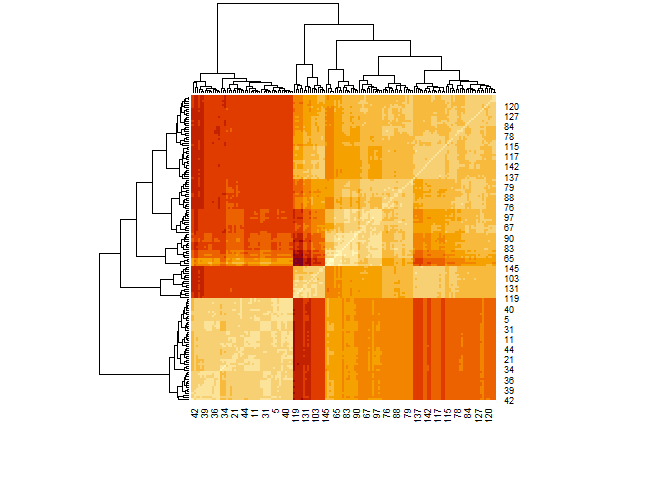
\includegraphics{internetaddiction_files/figure-latex/unnamed-chunk-15-1.pdf}

\begin{Shaded}
\begin{Highlighting}[]
\KeywordTok{ggcorrplot}\NormalTok{(r, }
           \DataTypeTok{hc.order =}\NormalTok{ T,}
           \DataTypeTok{type =} \StringTok{"lower"}\NormalTok{,}
           \DataTypeTok{lab =}\NormalTok{ T) }\CommentTok{#Visual diagram tangga  }
\end{Highlighting}
\end{Shaded}

\includegraphics{internetaddiction_files/figure-latex/unnamed-chunk-15-2.pdf}

\hypertarget{membuat-point-chart-korelasi-dari-variabel-internet-adiksi-dan-depresi-anxiety-dan-stress-dibedakan-dari-jenis-kelamin}{%
\subsection{\texorpdfstring{\emph{Membuat point chart korelasi dari
variabel internet adiksi dan depresi, anxiety, dan stress dibedakan dari
jenis
kelamin}}{Membuat point chart korelasi dari variabel internet adiksi dan depresi, anxiety, dan stress dibedakan dari jenis kelamin}}\label{membuat-point-chart-korelasi-dari-variabel-internet-adiksi-dan-depresi-anxiety-dan-stress-dibedakan-dari-jenis-kelamin}}

\begin{Shaded}
\begin{Highlighting}[]
\CommentTok{#Internet Addiction ~ Depression }
\NormalTok{ia_depres <-}\StringTok{ }\KeywordTok{ggplot}\NormalTok{(}\DataTypeTok{data =}\NormalTok{ internetdata, }
                    \KeywordTok{aes}\NormalTok{(}\DataTypeTok{x =}\NormalTok{ IA, }
                        \DataTypeTok{y =}\NormalTok{ Depresi,}
                        \DataTypeTok{color =}\NormalTok{ Sex)) }\OperatorTok{+}
\StringTok{  }\KeywordTok{geom_point}\NormalTok{(}\DataTypeTok{alpha =} \FloatTok{.7}\NormalTok{,}
             \DataTypeTok{size =} \DecValTok{3}\NormalTok{) }\OperatorTok{+}
\StringTok{  }\KeywordTok{geom_smooth}\NormalTok{(}\DataTypeTok{method =} \StringTok{"lm"}\NormalTok{, }
              \DataTypeTok{se =} \OtherTok{FALSE}\NormalTok{,}
              \DataTypeTok{size =} \FloatTok{1.5}\NormalTok{,}
              \DataTypeTok{col =} \StringTok{"black"}\NormalTok{) }\OperatorTok{+}
\StringTok{  }\KeywordTok{labs}\NormalTok{(}\DataTypeTok{y =} \StringTok{"Depresi"}\NormalTok{,}
       \DataTypeTok{x =} \StringTok{"Internet Addiction"}\NormalTok{, }
       \DataTypeTok{title =} \StringTok{"Korelasi Internet Addiction & Depresi"}\NormalTok{) }
\NormalTok{ia_depres}
\end{Highlighting}
\end{Shaded}

\begin{verbatim}
## `geom_smooth()` using formula 'y ~ x'
\end{verbatim}

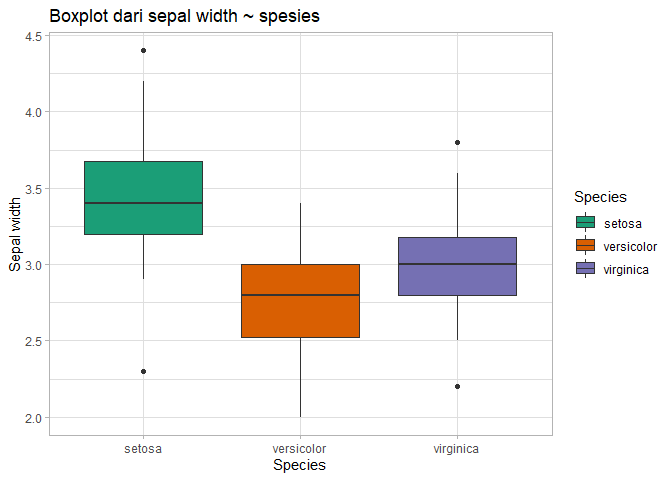
\includegraphics{internetaddiction_files/figure-latex/unnamed-chunk-16-1.pdf}

\begin{Shaded}
\begin{Highlighting}[]
\CommentTok{#Internet Addiction ~ Anxiety}
\NormalTok{ia_anxiety <-}\StringTok{ }\KeywordTok{ggplot}\NormalTok{(}\DataTypeTok{data =}\NormalTok{ internetdata, }
                    \KeywordTok{aes}\NormalTok{(}\DataTypeTok{x =}\NormalTok{ IA, }
                        \DataTypeTok{y =}\NormalTok{ Anxiety,}
                        \DataTypeTok{color =}\NormalTok{ Sex)) }\OperatorTok{+}
\StringTok{  }\KeywordTok{geom_point}\NormalTok{(}\DataTypeTok{alpha =} \FloatTok{.7}\NormalTok{,}
             \DataTypeTok{size =} \DecValTok{3}\NormalTok{) }\OperatorTok{+}
\StringTok{  }\KeywordTok{geom_smooth}\NormalTok{(}\DataTypeTok{method =} \StringTok{"lm"}\NormalTok{, }
              \DataTypeTok{se =} \OtherTok{FALSE}\NormalTok{,}
              \DataTypeTok{size =} \FloatTok{1.5}\NormalTok{,}
              \DataTypeTok{col =} \StringTok{"black"}\NormalTok{) }\OperatorTok{+}
\StringTok{  }\KeywordTok{labs}\NormalTok{(}\DataTypeTok{y =} \StringTok{"Anxiety"}\NormalTok{,}
       \DataTypeTok{x =} \StringTok{"Internet Addiction"}\NormalTok{, }
       \DataTypeTok{title =} \StringTok{"Korelasi Internet Addiction & Anxiety"}\NormalTok{) }
\NormalTok{ia_anxiety}
\end{Highlighting}
\end{Shaded}

\begin{verbatim}
## `geom_smooth()` using formula 'y ~ x'
\end{verbatim}

\includegraphics{internetaddiction_files/figure-latex/unnamed-chunk-16-2.pdf}

\begin{Shaded}
\begin{Highlighting}[]
\CommentTok{#Internet Addiction ~ Stress }
\NormalTok{ia_stress <-}\StringTok{ }\KeywordTok{ggplot}\NormalTok{(}\DataTypeTok{data =}\NormalTok{ internetdata, }
                    \KeywordTok{aes}\NormalTok{(}\DataTypeTok{x =}\NormalTok{ IA, }
                        \DataTypeTok{y =}\NormalTok{ Stress,}
                        \DataTypeTok{color =}\NormalTok{ Sex)) }\OperatorTok{+}
\StringTok{  }\KeywordTok{geom_point}\NormalTok{(}\DataTypeTok{alpha =} \FloatTok{.7}\NormalTok{,}
             \DataTypeTok{size =} \DecValTok{3}\NormalTok{) }\OperatorTok{+}
\StringTok{  }\KeywordTok{geom_smooth}\NormalTok{(}\DataTypeTok{method =} \StringTok{"lm"}\NormalTok{, }
              \DataTypeTok{se =} \OtherTok{FALSE}\NormalTok{,}
              \DataTypeTok{size =} \FloatTok{1.5}\NormalTok{,}
              \DataTypeTok{col =} \StringTok{"black"}\NormalTok{) }\OperatorTok{+}
\StringTok{  }\KeywordTok{labs}\NormalTok{(}\DataTypeTok{y =} \StringTok{"Stress"}\NormalTok{,}
       \DataTypeTok{x =} \StringTok{"Internet Addiction"}\NormalTok{, }
       \DataTypeTok{title =} \StringTok{"Korelasi Internet Addiction & Stress"}\NormalTok{) }
\NormalTok{ia_stress}
\end{Highlighting}
\end{Shaded}

\begin{verbatim}
## `geom_smooth()` using formula 'y ~ x'
\end{verbatim}

\includegraphics{internetaddiction_files/figure-latex/unnamed-chunk-16-3.pdf}

\hypertarget{uji-manova-menggunakan-kategori-ia-sebagai-variabel-independent}{%
\subsection{\texorpdfstring{\emph{Uji manova menggunakan kategori IA
sebagai variabel
independent}}{Uji manova menggunakan kategori IA sebagai variabel independent}}\label{uji-manova-menggunakan-kategori-ia-sebagai-variabel-independent}}

Pada penelitian ini, interent addiction merupakan variabel bebas
(independent variable) sedangkan depresi, anxiety, dan stres merupakan
variabel terikat (dependent variabel)

Uji statistik selanjutnya adalah menggunakan metode multivariate
analysis of variance. Hal ini memungkinkan kita menguji variabel
independen kategorial IA (adiksi dan nonadiksi) dengan variabel
dependent (depresi, anxiety, dan stress) untuk mengetahui apakah
terdapat perbedaan yang nyata pada kategori IA terhadap 3 variabel
dependent

\begin{Shaded}
\begin{Highlighting}[]
\CommentTok{# Prepare and Explore Data untuk Manova}

\NormalTok{manova_kat <-}\StringTok{ }\KeywordTok{select}\NormalTok{(internetdata, Depresi, Anxiety, Stress, Kategori)}
\NormalTok{manova_kat}\OperatorTok{$}\NormalTok{Kategori <-}\StringTok{ }\KeywordTok{factor}\NormalTok{(manova_kat}\OperatorTok{$}\NormalTok{Kategori, }\DataTypeTok{levels =} \KeywordTok{c}\NormalTok{(}\StringTok{"adiksi"}\NormalTok{, }\StringTok{"nonadiksi"}\NormalTok{))}

\CommentTok{#Pake library(rehsape2) untuk melt()}
\NormalTok{katmelt <-}\StringTok{ }\KeywordTok{melt}\NormalTok{(manova_kat, }\DataTypeTok{id =} \KeywordTok{c}\NormalTok{(}\StringTok{"Kategori"}\NormalTok{), }\DataTypeTok{measured =} \KeywordTok{c}\NormalTok{(}\StringTok{"Depresi"}\NormalTok{, }\StringTok{"Anxiety"}\NormalTok{, }\StringTok{"Stress"}\NormalTok{))}
\KeywordTok{names}\NormalTok{(katmelt) <-}\StringTok{ }\KeywordTok{c}\NormalTok{(}\StringTok{"Kategori"}\NormalTok{, }\StringTok{"Outcome_Measure"}\NormalTok{, }\StringTok{"Frequency"}\NormalTok{)}

\NormalTok{katmeltboxp <-}\StringTok{ }\NormalTok{katmelt }\OperatorTok
\StringTok{  }\KeywordTok{ggplot}\NormalTok{(}\KeywordTok{aes}\NormalTok{(Kategori, Frequency, }\DataTypeTok{col =}\NormalTok{ Outcome_Measure)) }\OperatorTok{+}
\StringTok{  }\KeywordTok{geom_boxplot}\NormalTok{() }\OperatorTok{+}
\StringTok{  }\KeywordTok{labs}\NormalTok{(}\DataTypeTok{x =} \StringTok{"Kategori Adiksi"}\NormalTok{,}
       \DataTypeTok{y =} \StringTok{"Jumlah Skor Depresi/Anxiety/Stress"}\NormalTok{,}
       \DataTypeTok{color =} \StringTok{"Outcome_Measure"}\NormalTok{) }\OperatorTok{+}
\StringTok{       }\KeywordTok{scale_y_continuous}\NormalTok{(}\DataTypeTok{breaks =} \KeywordTok{seq}\NormalTok{(}\DecValTok{0}\NormalTok{, }\DecValTok{60}\NormalTok{, }\DataTypeTok{by =} \DecValTok{2}\NormalTok{))}

\NormalTok{katmeltboxp}
\end{Highlighting}
\end{Shaded}

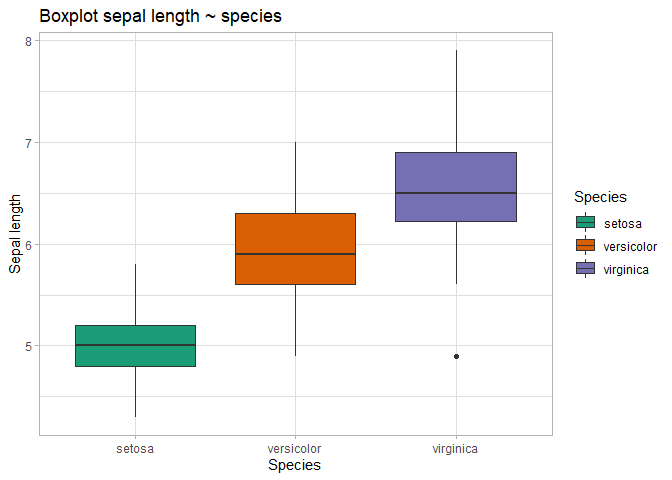
\includegraphics{internetaddiction_files/figure-latex/unnamed-chunk-17-1.pdf}

\hypertarget{analisis-manova}{%
\subsection{\texorpdfstring{\emph{Analisis
Manova}}{Analisis Manova}}\label{analisis-manova}}

Karena ini uji statistik, maka harus dibuat asumsi atau hipotesis
dasarnya dulu

Ho = Variabel depresi, anxiety, dan stres secara bersama-sama tidak
menunjukkan perbedaan nyata pada kategori ``adiksi'' dan ``noadiksi''
-atau bisa dikatakan, skor mean depresi, anxiety, dan stres sama pada
kategori adiksi dan nonadiksi

Ha = Variabel depresi, anxiety, dan stres secara bersama-sama
menunjukkan perbedaan nyata pada kategori ``adiksi'' dan ``nonadiksi''
-bisa juga dikatakan, skor mean depresi, anxiety, dan stres berbeda pada
kategori adiksi dan nonadiksi

\begin{Shaded}
\begin{Highlighting}[]
\NormalTok{manoutcome <-}\StringTok{ }\KeywordTok{cbind}\NormalTok{(manova_kat}\OperatorTok{$}\NormalTok{Depresi, manova_kat}\OperatorTok{$}\NormalTok{Anxiety, manova_kat}\OperatorTok{$}\NormalTok{Stress)}
\NormalTok{adiksiModel <-}\StringTok{ }\KeywordTok{manova}\NormalTok{(manoutcome }\OperatorTok{~}\StringTok{ }\NormalTok{Kategori, }\DataTypeTok{data =}\NormalTok{ manova_kat)}
\KeywordTok{summary}\NormalTok{(adiksiModel, }\DataTypeTok{intercept =} \OtherTok{TRUE}\NormalTok{)}
\end{Highlighting}
\end{Shaded}

\begin{verbatim}
##              Df  Pillai approx F num Df den Df    Pr(>F)    
## (Intercept)   1 0.78405   534.94      3    442 < 2.2e-16 ***
## Kategori      1 0.14927    25.85      3    442 2.005e-15 ***
## Residuals   444                                             
## ---
## Signif. codes:  0 '***' 0.001 '**' 0.01 '*' 0.05 '.' 0.1 ' ' 1
\end{verbatim}

\begin{Shaded}
\begin{Highlighting}[]
\KeywordTok{summary}\NormalTok{(adiksiModel, }\DataTypeTok{intercept=}\OtherTok{TRUE}\NormalTok{, }\DataTypeTok{test=}\StringTok{"Wilks"}\NormalTok{) }
\end{Highlighting}
\end{Shaded}

\begin{verbatim}
##              Df   Wilks approx F num Df den Df    Pr(>F)    
## (Intercept)   1 0.21595   534.94      3    442 < 2.2e-16 ***
## Kategori      1 0.85073    25.85      3    442 2.005e-15 ***
## Residuals   444                                             
## ---
## Signif. codes:  0 '***' 0.001 '**' 0.01 '*' 0.05 '.' 0.1 ' ' 1
\end{verbatim}

\begin{Shaded}
\begin{Highlighting}[]
\KeywordTok{summary}\NormalTok{(adiksiModel, }\DataTypeTok{intercept=}\OtherTok{TRUE}\NormalTok{, }\DataTypeTok{test=}\StringTok{"Hotelling"}\NormalTok{)}
\end{Highlighting}
\end{Shaded}

\begin{verbatim}
##              Df Hotelling-Lawley approx F num Df den Df    Pr(>F)    
## (Intercept)   1           3.6308   534.94      3    442 < 2.2e-16 ***
## Kategori      1           0.1755    25.85      3    442 2.005e-15 ***
## Residuals   444                                                      
## ---
## Signif. codes:  0 '***' 0.001 '**' 0.01 '*' 0.05 '.' 0.1 ' ' 1
\end{verbatim}

\begin{Shaded}
\begin{Highlighting}[]
\KeywordTok{summary}\NormalTok{(adiksiModel, }\DataTypeTok{intercept=}\OtherTok{TRUE}\NormalTok{, }\DataTypeTok{test=}\StringTok{"Roy"}\NormalTok{)}
\end{Highlighting}
\end{Shaded}

\begin{verbatim}
##              Df    Roy approx F num Df den Df    Pr(>F)    
## (Intercept)   1 3.6308   534.94      3    442 < 2.2e-16 ***
## Kategori      1 0.1755    25.85      3    442 2.005e-15 ***
## Residuals   444                                            
## ---
## Signif. codes:  0 '***' 0.001 '**' 0.01 '*' 0.05 '.' 0.1 ' ' 1
\end{verbatim}

\textbf{\emph{Catatan}}

\begin{itemize}
\item
  Tes dilakukan menggunakan prosedur Pillai (0.15), Wilks (0.85),
  Hotelling (0.18), dan Roy (0.18). Semua prosedur menunjukkan angka
  signifikansi \textless{} 0.05 (note: 2.2e-16 = 0.00000000000000022,
  dengan 15 nol setelah titik)
\item
  Dengan demikian maka Ho ditolak = Variabel depresi, anxiety, dan stres
  secara bersama-sama menunjukkan tingkat perbedaan yang nyata pada
  kategori adiksi (Mungkin saja responden dengan kategori adiksi
  internet lebih mungkin mengalami depresi, anxiety, dan stress,
  dibandingkan mereka yang berada dalam kategori nonadiksi)
\end{itemize}

\hypertarget{follow-up-analysis-univariate-test-statistics}{%
\subsection{\texorpdfstring{\emph{Follow-up analysis: univariate test
statistics}}{Follow-up analysis: univariate test statistics}}\label{follow-up-analysis-univariate-test-statistics}}

\begin{Shaded}
\begin{Highlighting}[]
\CommentTok{#Simply dengan memanggil }
\KeywordTok{summary.aov}\NormalTok{(adiksiModel)}
\end{Highlighting}
\end{Shaded}

\begin{verbatim}
##  Response 1 :
##              Df  Sum Sq Mean Sq F value    Pr(>F)    
## Kategori      1  1513.2 1513.17  39.543 7.689e-10 ***
## Residuals   444 16990.5   38.27                      
## ---
## Signif. codes:  0 '***' 0.001 '**' 0.01 '*' 0.05 '.' 0.1 ' ' 1
## 
##  Response 2 :
##              Df  Sum Sq Mean Sq F value    Pr(>F)    
## Kategori      1  2874.7 2874.65  67.369 2.466e-15 ***
## Residuals   444 18945.7   42.67                      
## ---
## Signif. codes:  0 '***' 0.001 '**' 0.01 '*' 0.05 '.' 0.1 ' ' 1
## 
##  Response 3 :
##              Df  Sum Sq Mean Sq F value    Pr(>F)    
## Kategori      1  3912.1  3912.1  69.594 9.277e-16 ***
## Residuals   444 24958.7    56.2                      
## ---
## Signif. codes:  0 '***' 0.001 '**' 0.01 '*' 0.05 '.' 0.1 ' ' 1
\end{verbatim}

\textbf{\emph{Catatan}}

\begin{itemize}
\item
  Tabel berlabel Respon 1 untuk variabel Depresi, Respon 2 untuk
  variabel Anxiety, dan Respon 3 untuk variabel Stress.
\item
  Perhatikan bahwa nilai F dan nilai p dari analisis follow-up MANOVA
  ini identik dengan yang diperoleh jika dilakukan analisa one-way ANOVA
  pada setiap variabel dependen.
\item
  Nilai p menunjukkan bahwa terdapat perbedaan yang signifikan antara
  kelompok terapi dalam hal Depresi, Anxiety, dan Stress (p \textless{}
  .05)
\end{itemize}

\end{document}
